\documentclass[11pt,letterpaper,openany]{book}
\usepackage[top=1in,bottom=1.2in,left=1.2in,right=1in,headheight=14pt]{geometry}
\usepackage{amsmath,amssymb,amsthm}
\usepackage{graphicx}
\usepackage{xcolor}
\usepackage{fancyhdr}
\usepackage{tikz}
\usepackage{pgfplots}
\usepackage{array}
\usepackage{booktabs}
\usepackage{multicol}
\usepackage{wallpaper}
\usepackage{lettrine}
\usepackage{contour}
\usepackage{background}
\usepackage[T1]{fontenc}

% Custom first letter command (simpler than lettrine)
\newcommand{\firstletter}[1]{%
    \textcolor{bloodred}{\fontsize{48}{48}\selectfont\bfseries #1}%
}

\usetikzlibrary{shapes.geometric,arrows.meta,decorations.pathmorphing,patterns,calc,shadows}
\pgfplotsset{compat=1.17}

% Fantasy color scheme
\definecolor{parchment}{RGB}{252,245,230}
\definecolor{bloodred}{RGB}{139,0,0}
\definecolor{goldink}{RGB}{218,165,32}
\definecolor{dragongreen}{RGB}{0,100,0}
\definecolor{mysticblue}{RGB}{25,25,112}
\definecolor{shadowgray}{RGB}{70,70,70}

% Set page color
\pagecolor{parchment}

% Background decoration - subtle corner ornaments
\backgroundsetup{
scale=1,
angle=0,
opacity=0.05,
contents={%

\begin{tikzpicture}[remember picture,overlay]
    % Corner ornaments using TikZ instead of external images
    \foreach \corner in {north west, north east, south west, south east} {
        \begin{scope}[shift={(current page.\corner)}]
            \draw[goldink!30, ultra thick] 
                (0,0) -- (2,0) (0,0) -- (0,-2)
                (0.5,0) -- (0.5,-0.5) -- (0,-0.5)
                (1,0) -- (1,-1) -- (0,-1)
                (1.5,0) -- (1.5,-1.5) -- (0,-1.5);
        \end{scope}
    }
\end{tikzpicture}
}
}

% Custom commands for fantasy styling
\newcommand{\fantasyquote}[1]{%
\begin{center}
\textit{\large #1}
\end{center}
}

\newcommand{\spell}[1]{\textcolor{mysticblue}{\textit{#1}}}
\newcommand{\ability}[1]{\textcolor{dragongreen}{\textbf{#1}}}
\newcommand{\damage}[1]{\textcolor{bloodred}{\textbf{#1}}}

% Fancy chapter styling
\usepackage{titlesec}
\titleformat{\chapter}[display]
{\normalfont\huge\bfseries\color{bloodred}}
{\chaptertitlename\ \thechapter}
{20pt}
{\Huge}

% Header and footer
\pagestyle{fancy}
\fancyhf{}
\fancyhead[LE,RO]{\thepage}
\fancyhead[LO]{\rightmark}
\fancyhead[RE]{\leftmark}
\renewcommand{\headrulewidth}{2pt}
\renewcommand{\footrulewidth}{1pt}

\begin{document}
\raggedbottom

% Foreword
\frontmatter
\chapter*{Foreword}

\firstletter{G}reetings, adventurer. Within these pages lies knowledge gathered over centuries by the greatest minds of the realms—wizards who plumbed the depths of arcane theory, warriors who studied the art of combat with mathematical precision, and scholars who documented the hidden patterns that govern our world.

This codex serves not merely as a collection of formulae and tables, but as a guide to understanding the very fabric of reality that underlies all adventures. From the humblest kobold warren to the mightiest dragon's lair, from the simplest cantrip to the most devastating ninth-level spell, all follow patterns that can be understood, predicted, and mastered.

\begin{center}
\textit{Knowledge is power. Power shared is power multiplied.}
\end{center}

May these teachings serve you well in your journeys.

\begin{flushright}
\textit{—Mordenkainen the Eternal}\\  
\textit{Circle of Eight}\\  
\textit{Free City of Greyhawk}
\end{flushright}

\chapter*{Introduction: How to Use This Codex}

\firstletter{T}his codex serves three masters: the player seeking mastery, the Dungeon Master crafting worlds, and the scholar understanding the deep patterns of adventure.

\section*{For Players}

Seek out chapters on:
\begin{itemize}
    \item \textbf{Combat Mechanics}: Understanding when to use your abilities for maximum impact
    \item \textbf{Character Optimization}: Building effective characters without falling into trap options
    \item \textbf{Action Economy}: Making every turn count
    \item \textbf{Magic Items}: Knowing what to seek and how to use it
\end{itemize}

\section*{For Dungeon Masters}

Focus on:
\begin{itemize}
    \item \textbf{Encounter Design}: Balancing challenge and fun
    \item \textbf{World Building}: Creating believable fantasy economics
    \item \textbf{Villain Creation}: Making memorable antagonists
    \item \textbf{Campaign Pacing}: Managing resources and tension
\end{itemize}

\section*{For Theorycrafters}

Delve into:
\begin{itemize}
    \item \textbf{Multiclassing Mathematics}: Finding optimal breakpoints
    \item \textbf{Probability Analysis}: Understanding the edge cases
    \item \textbf{System Interactions}: Where rules create emergent complexity
    \item \textbf{Resource Management}: Long-term optimization strategies
\end{itemize}

\fantasyquote{"Knowledge is power. Power shared is power multiplied."}

% Title page
\clearpage
\begin{titlepage}
\begin{center}
\vspace*{2cm}

{\Huge\textbf{The Codex of}}\\[0.5cm]
{\Huge\textbf{Dungeon Mechanics}}\\[1cm]


\begin{tikzpicture}
    % D20 die
    \node[regular polygon,
          regular polygon sides=3,
          draw=goldink,
          fill=goldink!20,
          minimum size=4cm,
          ultra thick,
          rotate=180] (die) {};
    \node at (die.center) {\Huge\textbf{20}};
    
    % Decorative dragons
    \draw[ultra thick,goldink,decorate,decoration={snake,amplitude=3mm}] 
        (-3,0) .. controls (-2,1) and (2,1) .. (3,0);
    \draw[ultra thick,goldink,decorate,decoration={snake,amplitude=3mm}] 
        (-3,0) .. controls (-2,-1) and (2,-1) .. (3,0);
\end{tikzpicture}

\vspace{1cm}

{\Large\textit{A Comprehensive Guide to}}\\
{\Large\textit{Role-Playing Game Mechanics}}\\[2cm]

{\large Being a Treatise on the Mathematical}\\
{\large Foundations of Adventure}\\[1cm]

$\ast$ \quad \textit{Fifth Edition} \quad $\ast$\\[2cm]

{\large Scribed by the Order of the Polyhedral}\\
{\large Anno Domini MMXXV}

\end{center}
\end{titlepage}

% Table of Contents
\tableofcontents
\clearpage

% Begin main content
\mainmatter
\chapter{The Nature of Magic and Reality}

\firstletter{B}efore delving into the mathematical certainties that govern our world, one must understand the mystical forces that shape reality itself. Magic is not chaos—it is order of the highest form, following laws as immutable as those that govern the fall of an apple or the flight of an arrow.

\section{The Weave of Magic}

In the beginning, there was the Weave—an invisible lattice of energy that permeates all things. Every spell cast, every magical item forged, every supernatural ability draws upon this fundamental force. The Weave responds to will and word, gesture and component, but always within the bounds of its own nature.

\fantasyquote{"Magic is the art of circumventing the normal." —Elminster of Shadowdale}

\subsection{The Schools of Magic}

The eight schools of magic represent different ways of manipulating the Weave:

\begin{figure}[h]
\centering
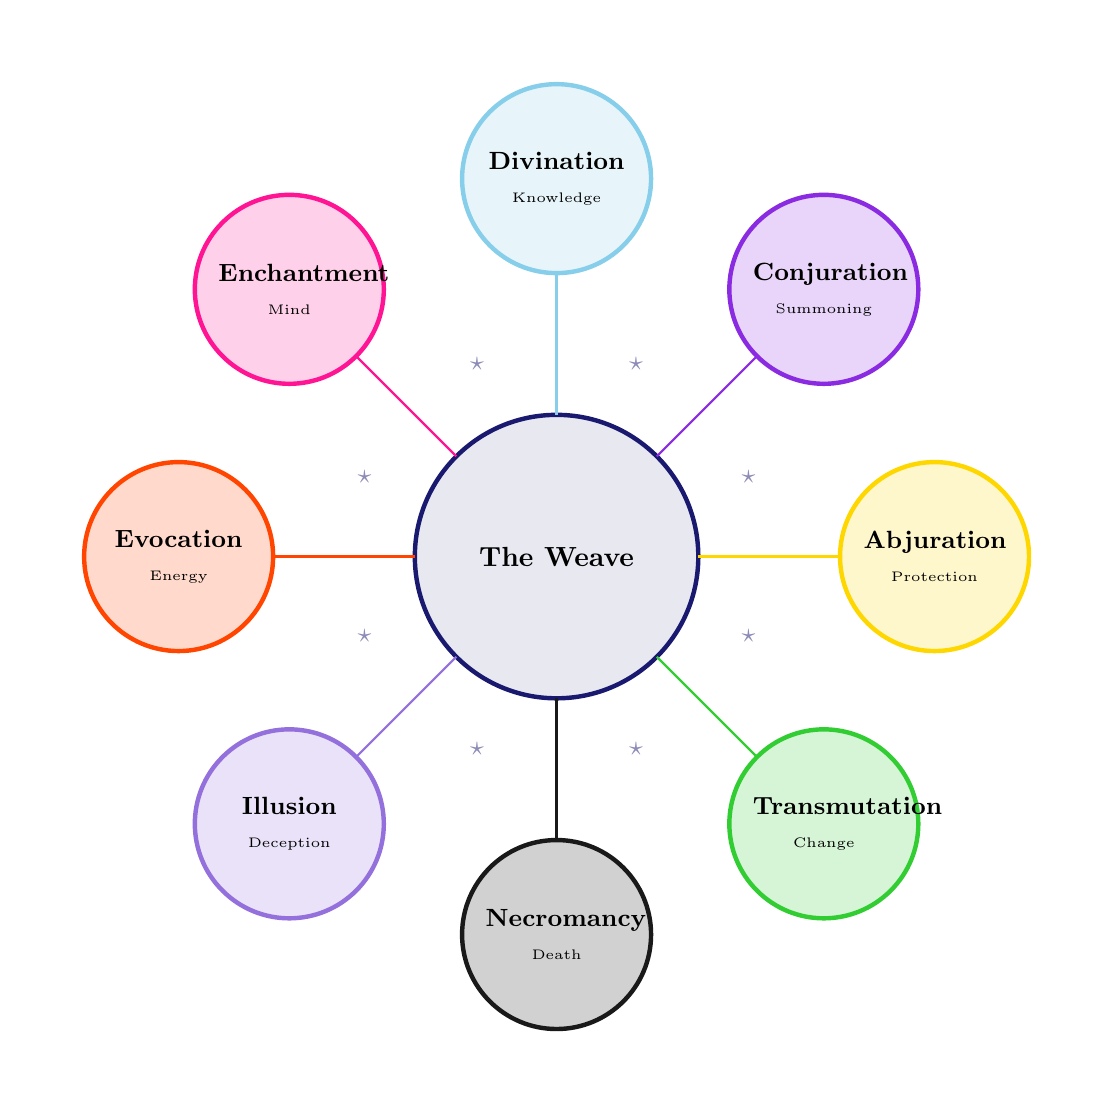
\begin{tikzpicture}[scale=1.2]
    % Define colors for each school
    \definecolor{abjcolor}{RGB}{255,215,0}  % Gold
    \definecolor{conjcolor}{RGB}{138,43,226} % Blue-violet
    \definecolor{divcolor}{RGB}{135,206,235} % Sky blue
    \definecolor{enchcolor}{RGB}{255,20,147} % Deep pink
    \definecolor{evocolor}{RGB}{255,69,0}    % Red-orange
    \definecolor{illcolor}{RGB}{147,112,219} % Medium purple
    \definecolor{neccolor}{RGB}{25,25,25}    % Near black
    \definecolor{trancolor}{RGB}{50,205,50}  % Lime green
    
    % Central Weave
    \draw[ultra thick, mysticblue, fill=mysticblue!10] (0,0) circle (1.5cm);
    \node at (0,0) {\textbf{The Weave}};
    
    % School nodes in octagon
    \foreach \i/\school/\col/\desc in {
        0/Abjuration/abjcolor/{Protection},
        45/Conjuration/conjcolor/{Summoning},
        90/Divination/divcolor/{Knowledge},
        135/Enchantment/enchcolor/{Mind},
        180/Evocation/evocolor/{Energy},
        225/Illusion/illcolor/{Deception},
        270/Necromancy/neccolor/{Death},
        315/Transmutation/trancolor/{Change}
    } {
        \begin{scope}[rotate=\i]
            % Connection to center
            \draw[\col, thick] (1.5,0) -- (3,0);
            % School circle
            \draw[\col, ultra thick, fill=\col!20] (4,0) circle (1cm);
            \node[text width=1.8cm, align=center] at (4,0) {\small\textbf{\school}\\\tiny\desc};
            % Spell examples
            \node[\col, font=\tiny] at (5.5,0) {\tiny};
        \end{scope}
    }
    
    % Add some decorative runes
    \foreach \angle in {22.5, 67.5, 112.5, 157.5, 202.5, 247.5, 292.5, 337.5} {
        \node[mysticblue!50] at (\angle:2.2cm) {$\star$};
    }
\end{tikzpicture}
\caption{The Eight Schools of Magic and Their Relationship to the Weave}
\end{figure}

\section{The Adventurer's Path}

Those who seek adventure follow paths worn by countless heroes before them. Yet each journey remains unique, shaped by choice and chance in equal measure.

\subsection{The Call to Adventure}

What transforms a baker into a barbarian? A scribe into a sorcerer? The call comes in many forms:
\begin{itemize}
    \item \textbf{Tragedy}: Your village burns, your family vanishes
    \item \textbf{Discovery}: You find a map, a sword, a spellbook
    \item \textbf{Destiny}: The prophecy speaks your name
    \item \textbf{Boredom}: Sometimes, the tavern life just isn't enough
\end{itemize}

\begin{figure}[h]
\centering
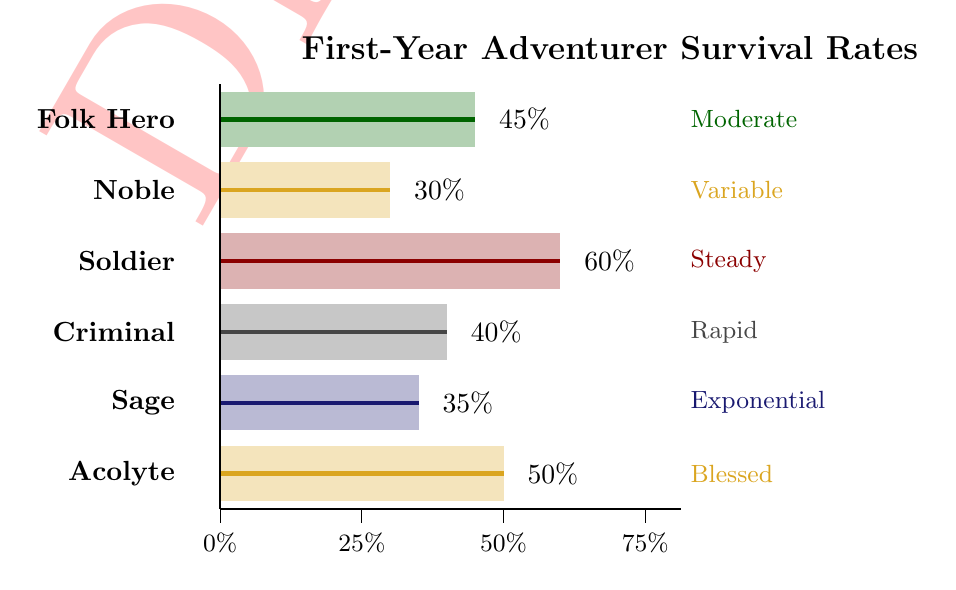
\begin{tikzpicture}[scale=0.9]
    % Title
    \node[font=\large\bfseries] at (6, 7) {First-Year Adventurer Survival Rates};
    
    % Draw survival rate bars
    \foreach \bg/\rate/\growth/\y/\col in {
        {Folk Hero}/45/{Moderate}/6/dragongreen,
        {Noble}/30/{Variable}/5/goldink,
        {Soldier}/60/{Steady}/4/bloodred,
        {Criminal}/40/{Rapid}/3/shadowgray,
        {Sage}/35/{Exponential}/2/mysticblue,
        {Acolyte}/50/{Blessed}/1/goldink%
    } {
        % Background label
        \node[anchor=east] at (0,\y) {\textbf{\bg}};
        
        % Survival rate bar
        \draw[\col!30, line width=20pt] (0.5,\y) -- (0.5+\rate*0.08,\y);
        \draw[\col, ultra thick] (0.5,\y) -- (0.5+\rate*0.08,\y);
        
        % Percentage label
        \node[anchor=west] at (0.5+\rate*0.08+0.2,\y) {\rate\%};
        
        % Growth type
        \node[anchor=west, \col, font=\small] at (7,\y) {\growth};
    }
    
    % Axes
    \draw[thick] (0.5,0.5) -- (0.5,6.5);
    \draw[thick] (0.5,0.5) -- (7,0.5);
    
    % Scale
    \foreach \x/\label in {0.5/0, 2.5/25, 4.5/50, 6.5/75} {
        \draw (\x,0.5) -- (\x,0.3);
        \node[below] at (\x,0.3) {\small\label\%};
    }
\end{tikzpicture}
\caption{Adventurer Background Analysis: Survival and Growth Patterns}
\end{figure}

\subsection{The Dungeon Phenomenon}

Dungeons—those mysterious complexes that dot the landscape—follow their own logic. They are not merely abandoned structures but living ecosystems that seem to generate both treasure and danger in mathematical proportion.

The Dungeon Equilibrium Theorem states:
\begin{equation}
\frac{\text{Treasure Value}}{\text{Danger Level}} = k \times \log(\text{Depth})
\end{equation}

Where $k$ is the dungeon constant, typically ranging from 100 to 500 gold pieces per challenge rating.

\section{The Planes of Existence}

Reality extends far beyond the Material Plane. Each plane operates according to its own mathematical constants:

\begin{itemize}
    \item \textbf{The Feywild}: Where time flows at $t_{\text{fey}} = t_{\text{material}} \times d100 / 50$
    \item \textbf{The Shadowfell}: Where emotions are dampened by factor 0.3
    \item \textbf{The Elemental Planes}: Where one element dominates at 95\% concentration
    \item \textbf{The Outer Planes}: Where alignment determines physics itself
\end{itemize}

\chapter{The Fundamentals of Chance}

\firstletter{I}n the realm of adventure, fate is determined by the roll of dice. Understanding the mathematics behind these random events separates the wise from the foolish, the living from the dead.

\fantasyquote{"The dice remember everything." - Ancient Gambler's Proverb}

\section{When Dice Tell Stories}

\subsection{The Sacred d20}

The twenty-sided die is more than a randomizer—it is fate's arbiter. While each face appears with equal frequency over thousands of rolls, in the moment of decision, probability becomes destiny.

\fantasyquote{"I've seen a peasant fell a giant with a lucky throw, and watched legends die to a goblin's crude blade. The dice care nothing for reputation." —Captain Marcus Ironside}

\subsection{The Drama of Extremes}

What matters is not the uniform distribution, but the moments when the dice create legends:
\begin{itemize}
    \item A natural 20 (5\% chance) transforms failure into triumph
    \item A natural 1 (5\% chance) humbles the mightiest hero
    \item The middle values (2-19) tell the story of skill and planning
\end{itemize}

\subsection{The Bell Curve of Heroism}

Multiple dice create reliability—the bell curve that separates wild chance from consistent performance. This is why:
\begin{itemize}
    \item Rogues stake everything on a single d20 attack roll
    \item Wizards rely on multiple d6s for \spell{fireball}—more predictable devastation
    \item Greatsword fighters (2d6) choose consistency over the greataxe's (1d12) variance
\end{itemize}

\textbf{Practical Wisdom}: When you need reliability, roll more dice. When you need miracles, roll fewer.

\section{Advantage and Disadvantage}

The mechanic of rolling twice and taking the higher (advantage) or lower (disadvantage) result fundamentally alters probabilities:

\begin{align}
P(\text{Advantage} \geq k) &= 1 - \left(\frac{k-1}{20}\right)^2 \\
P(\text{Disadvantage} \geq k) &= \left(\frac{21-k}{20}\right)^2
\end{align}

\begin{figure}[h]
\centering
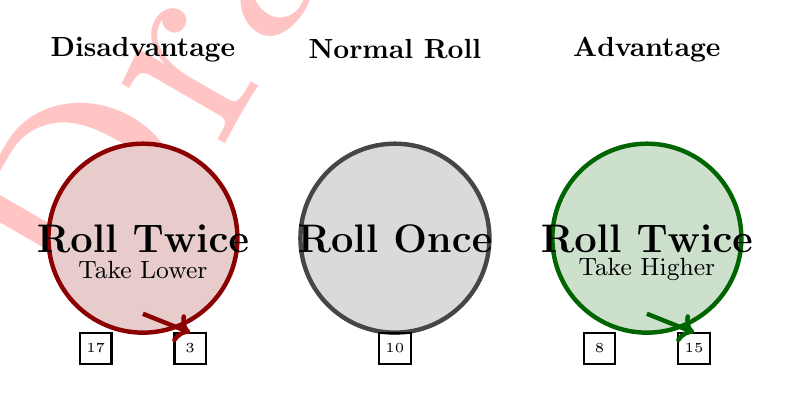
\begin{tikzpicture}[scale=0.8]
    % Visual representation of advantage/disadvantage
    \begin{scope}[shift={(-4,0)}]
        \node[font=\bfseries] at (0,3) {Disadvantage};
        \draw[bloodred, ultra thick, fill=bloodred!20] (0,0) circle (1.5cm);
        \node at (0,0) {\Large\textbf{Roll Twice}};
        \node at (0,-0.5) {\small Take Lower};
        
        % Example dice
        \draw[thick] (-1,-2) rectangle (-0.5,-1.5);
        \node at (-0.75,-1.75) {\tiny 17};
        \draw[thick] (0.5,-2) rectangle (1,-1.5);
        \node at (0.75,-1.75) {\tiny 3};
        \draw[bloodred, ultra thick, ->] (0,-1.2) -- (0.75,-1.5);
    \end{scope}
    
    \begin{scope}
        \node[font=\bfseries] at (0,3) {Normal Roll};
        \draw[shadowgray, ultra thick, fill=shadowgray!20] (0,0) circle (1.5cm);
        \node at (0,0) {\Large\textbf{Roll Once}};
        
        % Example die
        \draw[thick] (-0.25,-2) rectangle (0.25,-1.5);
        \node at (0,-1.75) {\tiny 10};
    \end{scope}
    
    \begin{scope}[shift={(4,0)}]
        \node[font=\bfseries] at (0,3) {Advantage};
        \draw[dragongreen, ultra thick, fill=dragongreen!20] (0,0) circle (1.5cm);
        \node at (0,0) {\Large\textbf{Roll Twice}};
        \node at (0,-0.5) {\small Take Higher};
        
        % Example dice
        \draw[thick] (-1,-2) rectangle (-0.5,-1.5);
        \node at (-0.75,-1.75) {\tiny 8};
        \draw[thick] (0.5,-2) rectangle (1,-1.5);
        \node at (0.75,-1.75) {\tiny 15};
        \draw[dragongreen, ultra thick, ->] (0,-1.2) -- (0.75,-1.5);
    \end{scope}
\end{tikzpicture}
\caption{Visual Guide to Advantage and Disadvantage Mechanics}
\end{figure}

\begin{figure}[h]
\centering
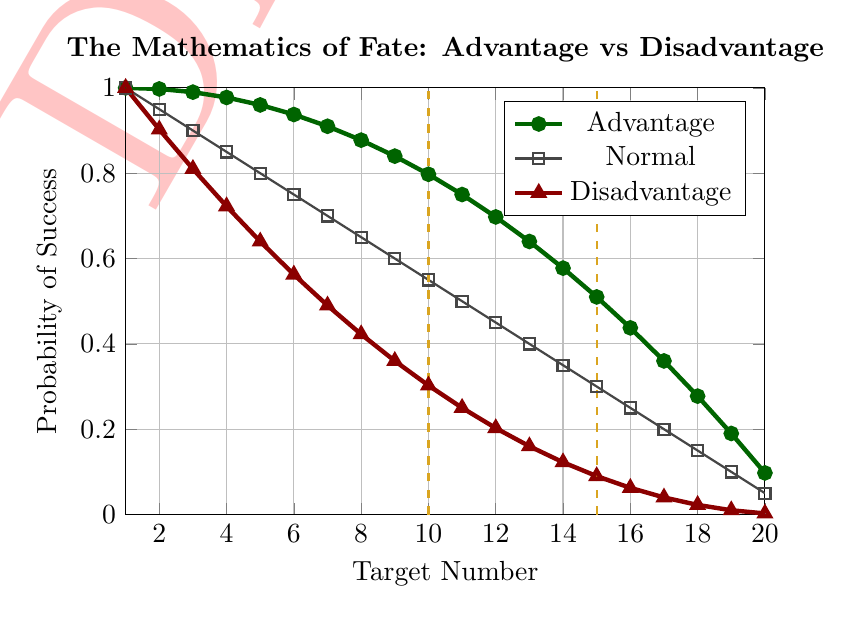
\begin{tikzpicture}
\begin{axis}[
    xlabel={Target Number},
    ylabel={Probability of Success},
    xmin=1, xmax=20,
    ymin=0, ymax=1,
    legend pos=north east,
    grid=major,
    width=0.8\textwidth,
    height=7cm,
    title={\textbf{The Mathematics of Fate: Advantage vs Disadvantage}}
]
\addplot[color=dragongreen,ultra thick,mark=*,mark size=2pt] coordinates {
    (1,1) (2,0.9975) (3,0.99) (4,0.9775) (5,0.96)
    (6,0.9375) (7,0.91) (8,0.8775) (9,0.84)
    (10,0.7975) (11,0.75) (12,0.6975) (13,0.64)
    (14,0.5775) (15,0.51) (16,0.4375) (17,0.36)
    (18,0.2775) (19,0.19) (20,0.0975)
};
\addlegendentry{Advantage}

\addplot[color=shadowgray,thick,mark=square,mark size=2pt] coordinates {
    (1,1) (2,0.95) (3,0.9) (4,0.85) (5,0.8)
    (6,0.75) (7,0.7) (8,0.65) (9,0.6)
    (10,0.55) (11,0.5) (12,0.45) (13,0.4)
    (14,0.35) (15,0.3) (16,0.25) (17,0.2)
    (18,0.15) (19,0.1) (20,0.05)
};
\addlegendentry{Normal}

\addplot[color=bloodred,ultra thick,mark=triangle,mark size=2pt] coordinates {
    (1,1) (2,0.9025) (3,0.81) (4,0.7225) (5,0.64)
    (6,0.5625) (7,0.49) (8,0.4225) (9,0.36)
    (10,0.3025) (11,0.25) (12,0.2025) (13,0.16)
    (14,0.1225) (15,0.09) (16,0.0625) (17,0.04)
    (18,0.0225) (19,0.01) (20,0.0025)
};
\addlegendentry{Disadvantage}

% Add key threshold lines
\draw[dashed, thick, goldink] (axis cs:10,0) -- (axis cs:10,1);
\node[goldink, font=\small, anchor=south] at (axis cs:10,1) {DC 10};
\draw[dashed, thick, goldink] (axis cs:15,0) -- (axis cs:15,1);
\node[goldink, font=\small, anchor=south] at (axis cs:15,1) {DC 15};
\end{axis}
\end{tikzpicture}
\caption{The Triforce of Probability: How Advantage Shapes Destiny}
\end{figure}

\chapter{Combat Mechanics}

\firstletter{W}hen blade meets flesh and spell meets shield, understanding the mathematics of combat can mean the difference between victory and defeat.

\section{Attack Resolution}

The basic attack formula:
\begin{equation}
\text{Attack Roll} = d20 + \text{Ability Modifier} + \text{Proficiency Bonus}
\end{equation}

Success occurs when:
\begin{equation}
\text{Attack Roll} \geq \text{Armor Class}
\end{equation}

\subsection{Critical Hits}

A natural 20 always hits and deals double damage dice:
\begin{equation}
\damage{Critical Damage} = 2 \times \text{Weapon Dice} + \text{Ability Modifier}
\end{equation}

\begin{figure}[h]
\centering
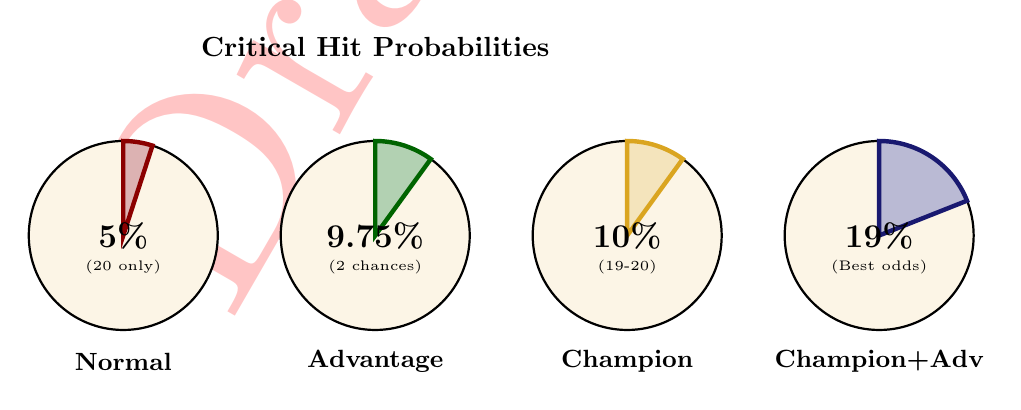
\begin{tikzpicture}[scale=0.8]
    % Title
    \node[font=\bfseries] at (0,5) {Critical Hit Probabilities};
    
    % Normal d20
    \begin{scope}[shift={(-4,2)}]
        \draw[thick, fill=parchment] (0,0) circle (1.5cm);
        \draw[bloodred, ultra thick, fill=bloodred!30] (0,0) -- (0,1.5) arc (90:72:1.5) -- cycle;
        \node[font=\small\bfseries] at (0,-2) {Normal};
        \node[font=\large\bfseries] at (0,0) {5\%};
        \node[font=\tiny] at (0,-0.5) {(20 only)};
    \end{scope}
    
    % Advantage
    \begin{scope}[shift={(0,2)}]
        \draw[thick, fill=parchment] (0,0) circle (1.5cm);
        \draw[dragongreen, ultra thick, fill=dragongreen!30] (0,0) -- (0,1.5) arc (90:54:1.5) -- cycle;
        \node[font=\small\bfseries] at (0,-2) {Advantage};
        \node[font=\large\bfseries] at (0,0) {9.75\%};
        \node[font=\tiny] at (0,-0.5) {(2 chances)};
    \end{scope}
    
    % Champion
    \begin{scope}[shift={(4,2)}]
        \draw[thick, fill=parchment] (0,0) circle (1.5cm);
        \draw[goldink, ultra thick, fill=goldink!30] (0,0) -- (0,1.5) arc (90:54:1.5) -- cycle;
        \node[font=\small\bfseries] at (0,-2) {Champion};
        \node[font=\large\bfseries] at (0,0) {10\%};
        \node[font=\tiny] at (0,-0.5) {(19-20)};
    \end{scope}
    
    % Champion with Advantage
    \begin{scope}[shift={(8,2)}]
        \draw[thick, fill=parchment] (0,0) circle (1.5cm);
        \draw[mysticblue, ultra thick, fill=mysticblue!30] (0,0) -- (0,1.5) arc (90:21.6:1.5) -- cycle;
        \node[font=\small\bfseries] at (0,-2) {Champion+Adv};
        \node[font=\large\bfseries] at (0,0) {19\%};
        \node[font=\tiny] at (0,-0.5) {(Best odds)};
    \end{scope}
\end{tikzpicture}
\caption{The Sweet Taste of Natural 20s}
\end{figure}

\section{The Art of War}

\subsection{Choosing Your Weapon}

Every weapon tells a story. The greatsword speaks of measured devastation, its 2d6 damage creating consistent results. The greataxe gambles on 1d12—same average damage, but with higher variance for those who court chaos.

\textbf{The Fighter's Dilemma}: With four attacks, small bonuses multiply:
\begin{itemize}
    \item A +1 weapon adds 4-8 damage per round
    \item \ability{Great Weapon Fighting} style adds $\approx 1.3$ damage per attack
    \item Action Surge doubles your impact for one glorious round
\end{itemize}

\fantasyquote{"The best swordsman in the world doesn't fear the second best. He fears the desperate fool with a dagger." —Master Alaric Swiftblade}

\subsection{Resistance and Vulnerability}

Damage modifiers affect the final damage:
\begin{align}
\text{Resisted Damage} &= \left\lfloor \frac{\text{Base Damage}}{2} \right\rfloor \\
\text{Vulnerable Damage} &= 2 \times \text{Base Damage}
\end{align}

\begin{figure}[h]
\centering
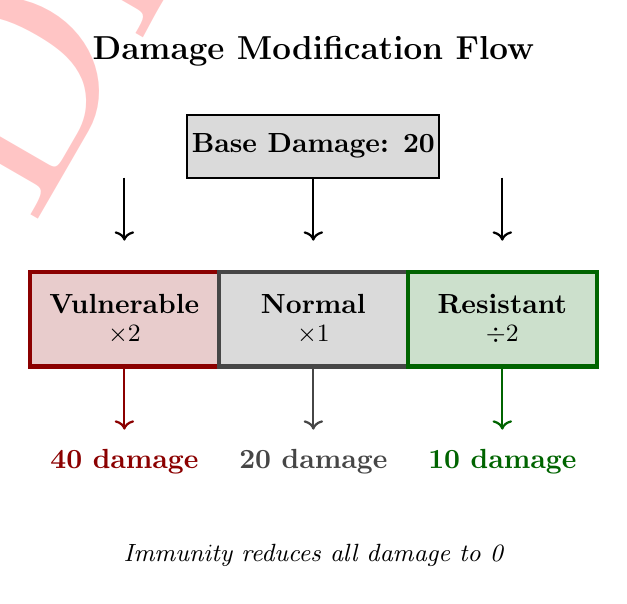
\begin{tikzpicture}[scale=0.8]
    % Title
    \node[font=\large\bfseries] at (0,5) {Damage Modification Flow};
    
    % Base damage
    \draw[thick, fill=shadowgray!20] (-2,3) rectangle (2,4);
    \node[font=\bfseries] at (0,3.5) {Base Damage: 20};
    
    % Three paths
    \draw[thick, ->] (-3,3) -- (-3,2);
    \draw[thick, ->] (0,3) -- (0,2);
    \draw[thick, ->] (3,3) -- (3,2);
    
    % Vulnerable
    \begin{scope}[shift={(-3,0)}]
        \draw[bloodred, ultra thick, fill=bloodred!20] (-1.5,0) rectangle (1.5,1.5);
        \node[font=\bfseries] at (0,1) {Vulnerable};
        \node[font=\small] at (0,0.5) {$\times 2$};
        \draw[bloodred, thick, ->] (0,0) -- (0,-1);
        \node[bloodred, font=\bfseries] at (0,-1.5) {40 damage};
    \end{scope}
    
    % Normal
    \begin{scope}[shift={(0,0)}]
        \draw[shadowgray, ultra thick, fill=shadowgray!20] (-1.5,0) rectangle (1.5,1.5);
        \node[font=\bfseries] at (0,1) {Normal};
        \node[font=\small] at (0,0.5) {$\times 1$};
        \draw[shadowgray, thick, ->] (0,0) -- (0,-1);
        \node[shadowgray, font=\bfseries] at (0,-1.5) {20 damage};
    \end{scope}
    
    % Resistant
    \begin{scope}[shift={(3,0)}]
        \draw[dragongreen, ultra thick, fill=dragongreen!20] (-1.5,0) rectangle (1.5,1.5);
        \node[font=\bfseries] at (0,1) {Resistant};
        \node[font=\small] at (0,0.5) {$\div 2$};
        \draw[dragongreen, thick, ->] (0,0) -- (0,-1);
        \node[dragongreen, font=\bfseries] at (0,-1.5) {10 damage};
    \end{scope}
    
    % Note about immunity
    \node[font=\small\itshape] at (0,-3) {Immunity reduces all damage to 0};
\end{tikzpicture}
\caption{How Damage Modifiers Work}
\end{figure}

\chapter{Magic and Spellcasting}

\firstletter{T}he arcane arts follow their own mathematical laws, binding reality to the will of the caster.

\section{Spell Save DCs}

The save DC represents the caster's mastery over the Weave itself. As you grow in power, reality bends more readily to your will:

\textbf{The Caster's Edge}:
\begin{itemize}
    \item Level 1-4: DC 13-14 (novice practitioners)
    \item Level 5-8: DC 15-16 (seasoned mages)
    \item Level 9-16: DC 17-18 (master spellcasters)
    \item Level 17-20: DC 19+ (reality's architects)
\end{itemize}

\fantasyquote{"A fireball doesn't ask permission. That's what the save is for." —Tasha}

\section{Spell Slot Progression}

Spellcasters gain slots according to their level, forming a mystical pyramid of power:

\begin{figure}[h]
\centering
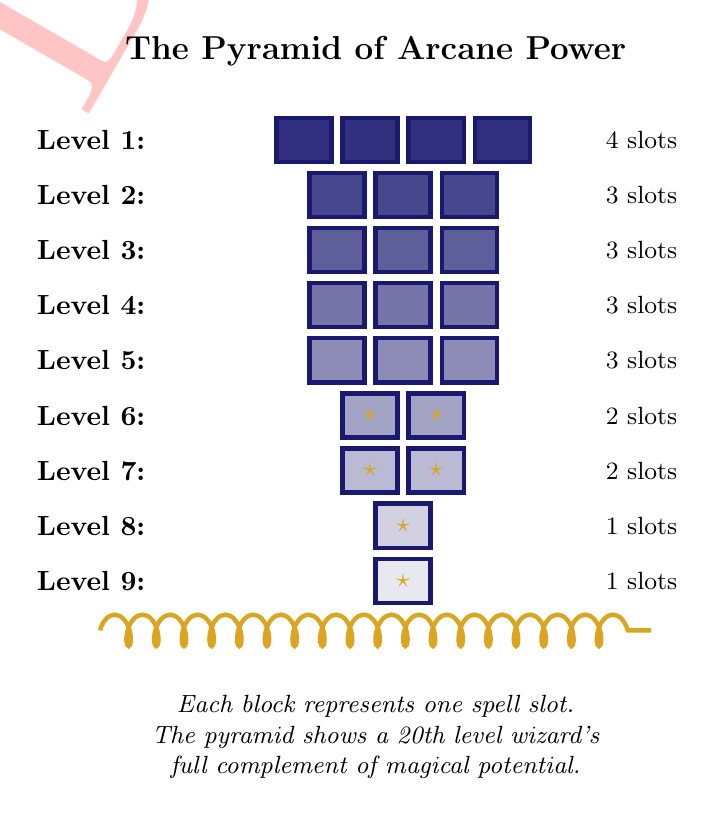
\begin{tikzpicture}[scale=0.7]
    % Title
    \node[font=\large\bfseries] at (0,10) {The Pyramid of Arcane Power};
    
    % Define slot counts for level 20
    \def\slots{{1,1,2,2,3,3,3,3,4}} % 9th to 1st level slots
    
    % Draw the pyramid
    \foreach \level in {1,...,9} {
        \pgfmathtruncatemacro{\slotcount}{\slots[9-\level]}
        \pgfmathsetmacro{\ypos}{9-\level}
        
        % Draw slot boxes
        \foreach \slot in {1,...,\slotcount} {
            \pgfmathsetmacro{\xpos}{(\slot-1)*1.2 - (\slotcount-1)*0.6}
            
            % Color gradient from low to high level
            \pgfmathsetmacro{\intensity}{100 - \level*10}
            \definecolor{slotcolor}{RGB}{25,25,\intensity}
            
            % Slot box
            \draw[ultra thick, mysticblue, fill=mysticblue!\intensity] 
                (\xpos,\ypos) rectangle (\xpos+1,\ypos+0.8);
            
            % Stars for higher level slots
            \ifnum\level>5
                \node[goldink] at (\xpos+0.5,\ypos+0.4) {$\star$};
            \fi
        }
        
        % Level label
        \node[anchor=east, font=\bfseries] at (-4,\ypos+0.4) {Level \level:};
        \node[anchor=west, font=\small] at (4,\ypos+0.4) {\slotcount\ slots};
    }
    
    % Add decorative elements
    \draw[goldink, ultra thick, decorate, decoration={coil,amplitude=2mm}] 
        (-5,-0.5) -- (5,-0.5);
    
    % Legend
    \node[below, text width=8cm, align=center, font=\small\itshape] at (0,-1.5) 
        {Each block represents one spell slot. The pyramid shows a 20th level wizard's\\full complement of magical potential.};
\end{tikzpicture}
\caption{Spell Slot Progression: The Pyramid of Power}
\end{figure}

\subsection{Multiclass Spell Slots}

For those who blend magical traditions, the pyramid shifts and adapts based on their combined mystical understanding.

\section{Area of Effect Calculations}

\subsection{Spell Areas Visualized}

\begin{figure}[h]
\centering
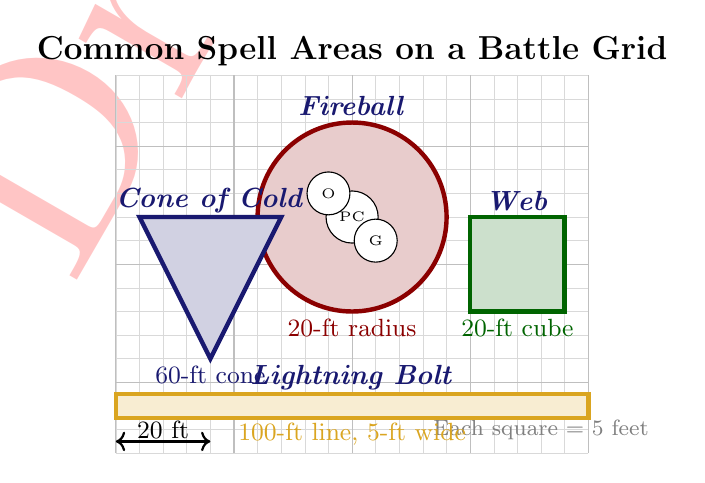
\begin{tikzpicture}[scale=0.3]
    % Grid (5-ft squares)
    \draw[step=1,gray!30,very thin] (-10,-8) grid (10,8);
    \draw[step=5,gray!50,thin] (-10,-8) grid (10,8);
    
    % Title
    \node[font=\large\bfseries] at (0,9) {Common Spell Areas on a Battle Grid};
    
    % Grid scale label
    \node[font=\footnotesize,gray] at (8,-7) {Each square = 5 feet};
    
    % Fireball (20-ft radius = 4 squares)
    \begin{scope}[shift={(0,2)}]
        \draw[bloodred, ultra thick, fill=bloodred!20] (0,0) circle (4);
        \node[bloodred, font=\bfseries] at (0,4.7) {\spell{Fireball}};
        \node[bloodred, font=\small] at (0,-4.7) {20-ft radius};
    \end{scope}
    
    % Web (20-ft cube = 4x4 squares)
    \begin{scope}[shift={(7,0)}]
        \draw[dragongreen, ultra thick, fill=dragongreen!20] (-2,-2) rectangle (2,2);
        \node[dragongreen, font=\bfseries] at (0,2.7) {\spell{Web}};
        \node[dragongreen, font=\small] at (0,-2.7) {20-ft cube};
    \end{scope}
    
    % Cone of Cold (60-ft cone)
    \begin{scope}[shift={(-6,-4)}]
        \draw[mysticblue, ultra thick, fill=mysticblue!20] 
            (0,0) -- (-3,6) -- (3,6) -- cycle;
        \node[mysticblue, font=\bfseries] at (0,6.7) {\spell{Cone of Cold}};
        \node[mysticblue, font=\small] at (0,-0.7) {60-ft cone};
    \end{scope}
    
    % Lightning Bolt (100-ft line = 20 squares, 5-ft wide)
    \begin{scope}[shift={(0,-6)}]
        \draw[goldink, ultra thick, fill=goldink!20] (-10,-0.5) rectangle (10,0.5);
        \node[goldink, font=\bfseries] at (0,1.2) {\spell{Lightning Bolt}};
        \node[goldink, font=\small] at (0,-1.2) {100-ft line, 5-ft wide};
    \end{scope}
    
    % Scale indicator
    \draw[thick, <->] (-10,-7.5) -- (-6,-7.5);
    \node[font=\small] at (-8,-7) {20 ft};
    
    % Example creatures for scale
    \node[font=\tiny,circle,draw,fill=white] at (0,2) {PC};
    \node[font=\tiny,circle,draw,fill=white] at (1,1) {G};
    \node[font=\tiny,circle,draw,fill=white] at (-1,3) {O};
\end{tikzpicture}
\caption{Spell Areas: Know Your Blast Radius}
\end{figure}

\chapter{Character Optimization}

\firstletter{T}o forge a legendary hero requires understanding the mathematical relationships between abilities, skills, and equipment.

\section{Ability Score Arrays}

Standard arrays and their point buy costs:

\begin{table}[h]
\centering
\begin{tabular}{@{}lcccccc@{}}
\toprule
\textbf{Method} & \multicolumn{6}{c}{\textbf{Scores}} \\
\midrule
Standard Array & 15 & 14 & 13 & 12 & 10 & 8 \\
Point Buy (27 pts) & 15 & 15 & 15 & 8 & 8 & 8 \\
Balanced & 14 & 14 & 14 & 11 & 10 & 9 \\
\bottomrule
\end{tabular}
\caption{Common Ability Arrays}
\end{table}

\section{The Boundaries of Power}

Bounded accuracy ensures that a goblin can still threaten a high-level hero, and a peasant militia might—just might—bring down a dragon. This is not a flaw but a feature.

\textbf{Why Numbers Stay Small}:
\begin{itemize}
    \item A 20th-level fighter still fears a mob
    \item Ancient dragons can fail saves against apprentice wizards
    \item Magic items remain meaningful at all levels
    \item The d20 always matters
\end{itemize}

\fantasyquote{"I've seen level 20 heroes die to falling rocks. Hubris is the greatest enemy." —Volo}

\subsection{To-Hit Probability}

Given a +X to hit against AC Y:
\begin{equation}
P(\text{hit}) = \frac{21 - (Y - X)}{20} \quad \text{clamped to } [0.05, 0.95]
\end{equation}

\subsection{Death Saving Throws}

\begin{figure}[h]
\centering
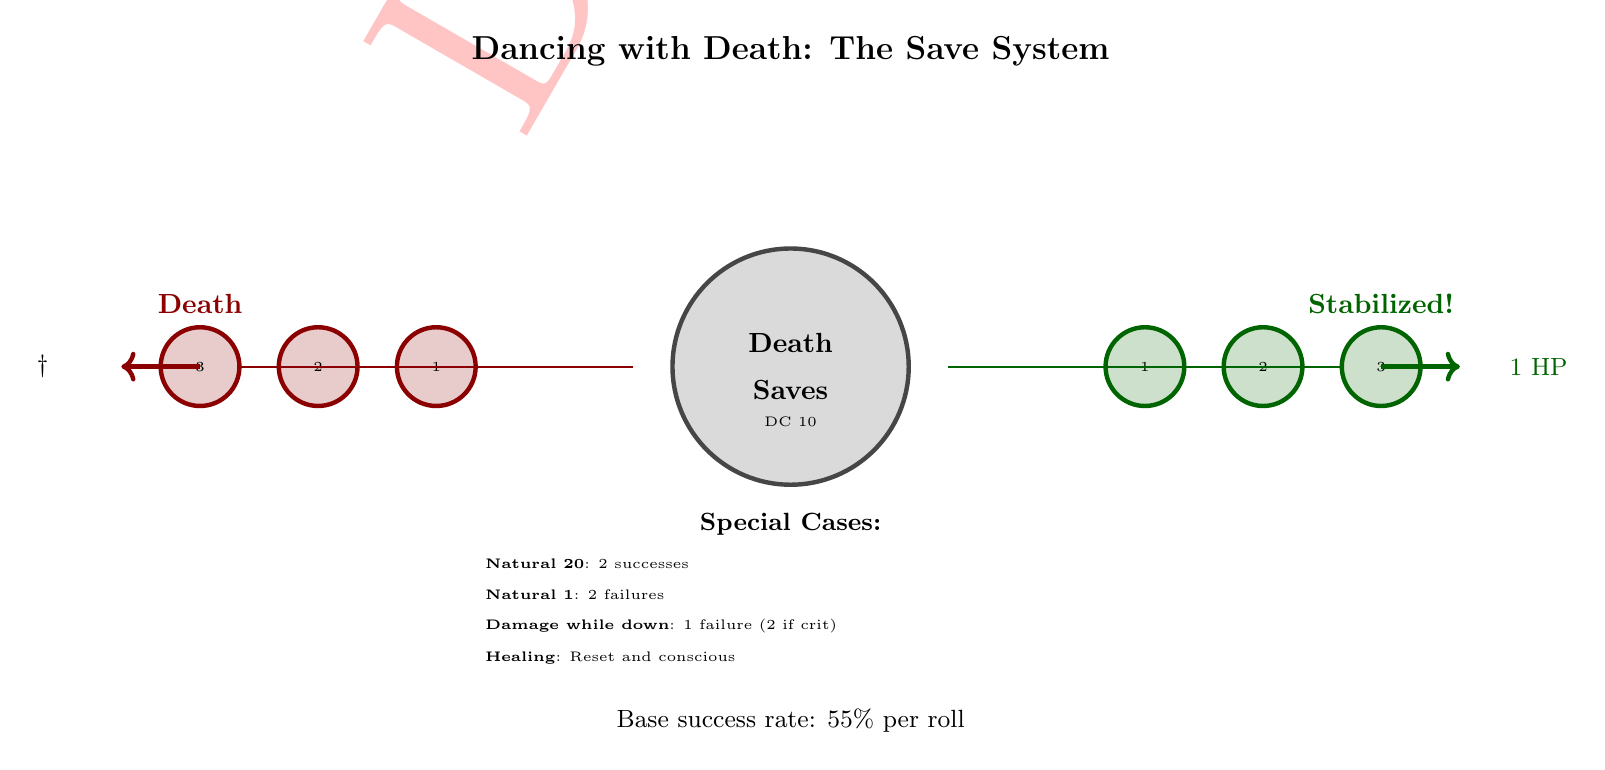
\begin{tikzpicture}[scale=1]
    % Title
    \node[font=\large\bfseries] at (0,6) {Dancing with Death: The Save System};
    
    % Central death figure
    \draw[shadowgray, ultra thick, fill=shadowgray!20] (0,2) circle (1.5cm);
    \node[font=\bfseries] at (0,2.3) {Death};
    \node[font=\bfseries] at (0,1.7) {Saves};
    \node[font=\tiny] at (0,1.3) {DC 10};
    
    % Success path (right)
    \foreach \i in {1,2,3} {
        \draw[dragongreen, thick] (2,2) -- (3+\i*1.5,2);
        \draw[dragongreen, ultra thick, fill=dragongreen!20] (3+\i*1.5,2) circle (0.5cm);
        \node[font=\tiny] at (3+\i*1.5,2) {\i};
    }
    \node[dragongreen, font=\bfseries] at (7.5,2.8) {Stabilized!};
    \draw[dragongreen, ultra thick, ->] (7.5,2) -- (8.5,2);
    \node[dragongreen, font=\small] at (9.5,2) {1 HP};
    
    % Failure path (left)  
    \foreach \i in {1,2,3} {
        \draw[bloodred, thick] (-2,2) -- (-3-\i*1.5,2);
        \draw[bloodred, ultra thick, fill=bloodred!20] (-3-\i*1.5,2) circle (0.5cm);
        \node[font=\tiny] at (-3-\i*1.5,2) {\i};
    }
    \node[bloodred, font=\bfseries] at (-7.5,2.8) {Death};
    \draw[bloodred, ultra thick, ->] (-7.5,2) -- (-8.5,2);
    \node[font=\small] at (-9.5,2) {$\dagger$};
    
    % Special cases
    \node[font=\small\bfseries] at (0,0) {Special Cases:};
    \node[font=\tiny, anchor=west] at (-4,-0.5) {\textbf{Natural 20}: 2 successes};
    \node[font=\tiny, anchor=west] at (-4,-0.9) {\textbf{Natural 1}: 2 failures};
    \node[font=\tiny, anchor=west] at (-4,-1.3) {\textbf{Damage while down}: 1 failure (2 if crit)};
    \node[font=\tiny, anchor=west] at (-4,-1.7) {\textbf{Healing}: Reset and conscious};
    
    % Probability
    \node[font=\small] at (0,-2.5) {Base success rate: 55\% per roll};
\end{tikzpicture}
\caption{Death Saves: Three Strikes and You're Out (or In)}
\end{figure}

\begin{figure}[h]
\centering
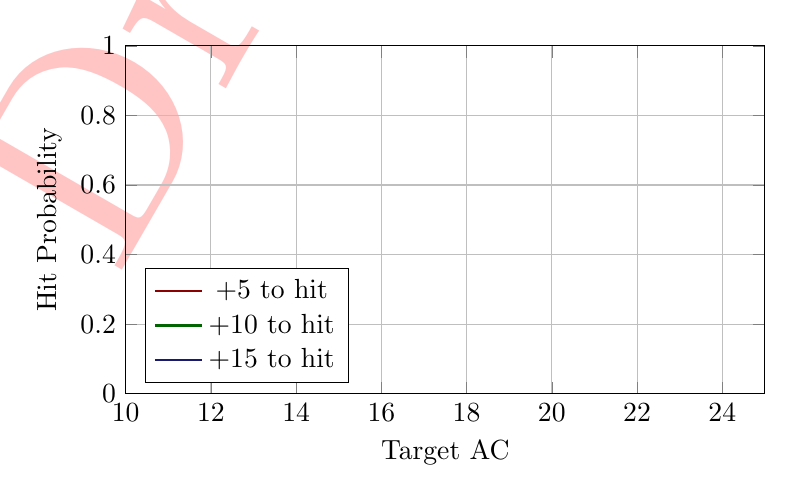
\begin{tikzpicture}
\begin{axis}[
    xlabel={Target AC},
    ylabel={Hit Probability},
    xmin=10, xmax=25,
    ymin=0, ymax=1,
    legend pos=south west,
    grid=major,
    width=0.8\textwidth,
    height=6cm
]
\addplot[color=bloodred,thick] {min(0.95, max(0.05, (21-(x-5))/20))};
\addlegendentry{+5 to hit}

\addplot[color=dragongreen,thick] {min(0.95, max(0.05, (21-(x-10))/20))};
\addlegendentry{+10 to hit}

\addplot[color=mysticblue,thick] {min(0.95, max(0.05, (21-(x-15))/20))};
\addlegendentry{+15 to hit}
\end{axis}
\end{tikzpicture}
\caption{Hit Probability by Attack Bonus}
\end{figure}

\chapter{Encounter Design}

\firstletter{B}alancing encounters requires understanding the mathematical relationships between party strength and monster challenge.

\section{Challenge Rating System}

Challenge Rating is a lie—a useful lie, but a lie nonetheless. CR assumes:
\begin{itemize}
    \item No magic items (ha!)
    \item No tactical advantage
    \item No optimization
    \item Average rolls
\end{itemize}

\textbf{Real CR Adjustments}:
\begin{itemize}
    \item Well-equipped party: CR +2
    \item Optimized party: CR +3
    \item Environmental advantage: CR -2
    \item Surprised/ambushed: CR +4
\end{itemize}

\subsection{The Deadly Encounter Paradox}

"Deadly" doesn't mean lethal—it means resource-draining. A truly deadly encounter:
\begin{itemize}
    \item Forces spell slot expenditure
    \item Threatens unconsciousness for 1-2 party members
    \item Cannot be solved by basic attacks alone
    \item Creates memorable stories
\end{itemize}

\textbf{The 6-8 Encounter Myth}: This assumes medium encounters. Most groups prefer:
\begin{itemize}
    \item 2-3 deadly encounters per day
    \item 1 short rest between
    \item More dramatic tension, less bookkeeping
\end{itemize}

\section{Action Economy}

The number of actions per side heavily influences difficulty:

\begin{equation}
\text{Effective CR} = \text{Base CR} \times \sqrt{\frac{\text{Monster Actions}}{\text{Party Actions}}}
\end{equation}

\subsection{Encounter Multipliers}

\begin{table}[h]
\centering
\begin{tabular}{@{}lc@{}}
\toprule
\textbf{Number of Monsters} & \textbf{Multiplier} \\
\midrule
1 & ×1 \\
2 & ×1.5 \\
3-6 & ×2 \\
7-10 & ×2.5 \\
11-14 & ×3 \\
15+ & ×4 \\
\bottomrule
\end{tabular}
\caption{Encounter Difficulty Multipliers}
\end{table}

\chapter{Treasures and Tribulations}

\firstletter{G}old flows like water through the hands of adventurers, and magic items become the milestones of a hero's journey.

\section{The Adventurer's Economy}

\subsection{Why Adventurers Are Rich}

The average commoner earns 1 sp per day. A single ancient red dragon's hoard contains approximately 300,000 gp. This economic disparity exists because:
\begin{itemize}
    \item Adventurers literally create wealth by clearing dungeons
    \item Magic items have no market—only adventurers can use them effectively
    \item The mortality rate ensures few collect their rewards
\end{itemize}

\subsection{The Magic Item Sweet Spot}

\begin{table}[h]
\centering
\begin{tabular}{@{}lcc@{}}
\toprule
\textbf{Character Level} & \textbf{Appropriate Rarity} & \textbf{Game Impact} \\
\midrule
1-4 & Common, Uncommon & Convenience and flavor \\
5-10 & Uncommon, Rare & Build-defining choices \\
11-16 & Rare, Very Rare & Campaign-shaping power \\
17-20 & Very Rare, Legendary & Reality-bending effects \\
\bottomrule
\end{tabular}
\caption{Magic Item Progression}
\end{table}

\section{Creating Legendary Campaigns}

\subsection{The Three Pillars in Practice}

\textbf{Combat} (40\% of play): Where mechanics meet drama
\begin{itemize}
    \item Average 3-4 rounds creates urgency
    \item One deadly encounter > three easy ones
    \item Environmental hazards multiply threat
\end{itemize}

\textbf{Exploration} (30\% of play): Where world-building lives
\begin{itemize}
    \item Meaningful choices, not endless corridors
    \item Resource depletion creates tension
    \item Discovery rewards clever thinking
\end{itemize}

\textbf{Social} (30\% of play): Where characters become people
\begin{itemize}
    \item NPCs want things the party can provide
    \item Reputation has mechanical benefits
    \item Not every problem has a violent solution
\end{itemize}

\chapter{Advanced Action Economy}

\firstletter{M}astery of the action economy separates novice adventurers from legendary heroes. Every second counts in the heat of battle.

\section{Action Types and Optimization}

Each turn, a character has access to:
\begin{itemize}
    \item 1 Action
    \item 1 Movement (up to speed)
    \item 1 Bonus Action (if available)
    \item 1 Reaction (if triggered)
    \item Unlimited free object interactions
\end{itemize}

\subsection{Expected Actions Per Combat}

Given average combat length of $L$ rounds:
\begin{equation}
E[\text{Total Actions}] = L \times (1 + P(\text{bonus}) + P(\text{reaction}))
\end{equation}

Where typical values:
\begin{itemize}
    \item $L \approx 3-4$ rounds
    \item $P(\text{bonus}) \approx 0.7$ for optimized builds
    \item $P(\text{reaction}) \approx 0.3$ per round
\end{itemize}

\begin{table}[h]
\centering
\begin{tabular}{@{}lccc@{}}
\toprule
\textbf{Class Feature} & \textbf{Action Cost} & \textbf{DPR Increase} & \textbf{Efficiency} \\
\midrule
Two-Weapon Fighting & Bonus & +3.5 to +6.5 & High \\
Polearm Master & Bonus & +2.5 to +6.5 & High \\
Cunning Action & Bonus & Defensive & Situational \\
Healing Word & Bonus & Negative DPR & Emergency \\
Hex/Hunter's Mark & Bonus (setup) & +3.5/turn & High \\
\bottomrule
\end{tabular}
\caption{Bonus Action Efficiency Analysis}
\end{table}

\section{Turn Optimization Mathematics}

\subsection{Optimal Action Selection}

Given multiple possible actions, optimize for expected value:
\begin{equation}
\text{Optimal Action} = \arg\max_i \left( P(\text{success}_i) \times V(\text{outcome}_i) \right)
\end{equation}

\begin{figure}[h]
\centering
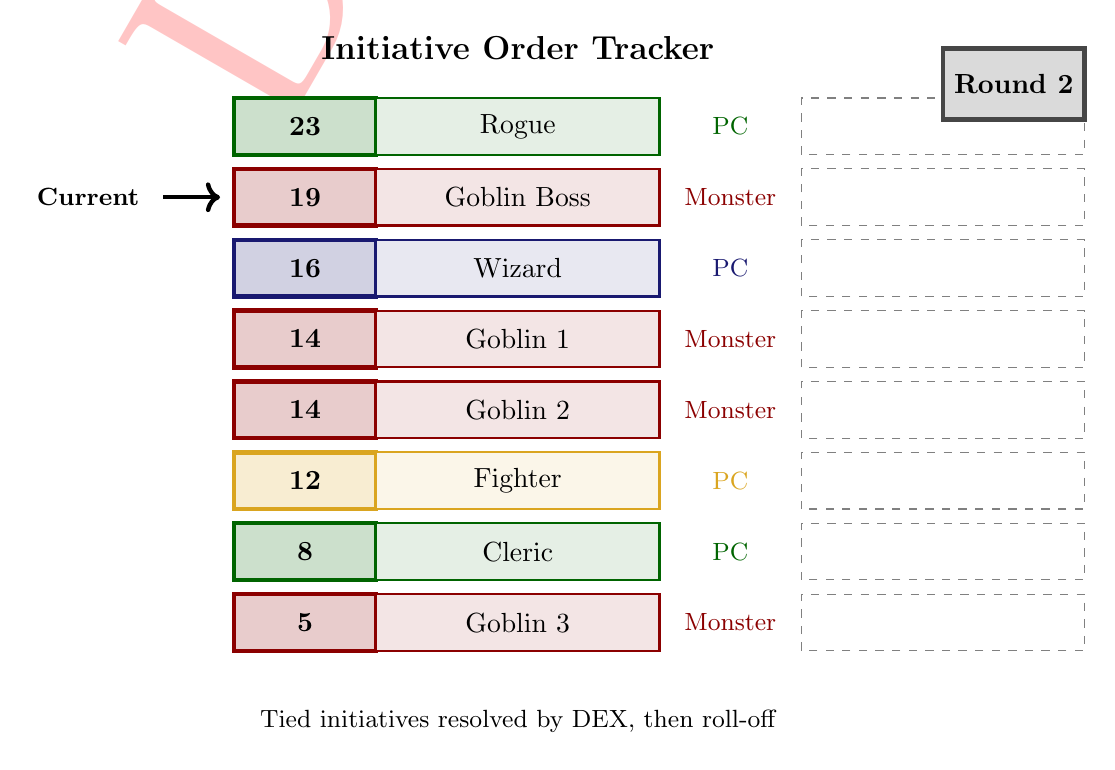
\begin{tikzpicture}[scale=0.9]
    % Title
    \node[font=\large\bfseries] at (0,8) {Initiative Order Tracker};
    
    % Initiative track
    \foreach \init/\name/\type/\col [count=\i] in {
        {23/{Rogue}/{PC}/dragongreen},
        {19/{Goblin Boss}/{Monster}/bloodred},
        {16/{Wizard}/{PC}/mysticblue},
        {14/{Goblin 1}/{Monster}/bloodred},
        {14/{Goblin 2}/{Monster}/bloodred},
        {12/{Fighter}/{PC}/goldink},
        {8/{Cleric}/{PC}/dragongreen},
        {5/{Goblin 3}/{Monster}/bloodred}%
    } {
        \pgfmathtruncatemacro{\ypos}{8 - \i}
        
        % Initiative box
        \draw[\col, ultra thick, fill=\col!20] (-4,\ypos-0.5) rectangle (-2,\ypos+0.3);
        \node[font=\bfseries] at (-3,\ypos-0.1) {\init};
        
        % Name box
        \draw[\col, thick, fill=\col!10] (-2,\ypos-0.5) rectangle (2,\ypos+0.3);
        \node at (0,\ypos-0.1) {\name};
        
        % Type indicator
        \node[\col, font=\small] at (3,\ypos-0.1) {\type};
        
        % Conditions/notes area
        \draw[gray, dashed] (4,\ypos-0.5) rectangle (8,\ypos+0.3);
    }
    
    % Current turn indicator (pointing to Wizard, row 3)
    \draw[ultra thick, ->] (-5,5.9) -- (-4.2,5.9);
    \node[font=\small\bfseries, anchor=east] at (-5.2,5.9) {Current};
    
    % Round counter
    \draw[shadowgray, ultra thick, fill=shadowgray!20] (6,7) rectangle (8,8);
    \node[font=\bfseries] at (7,7.5) {Round 2};
    
    % Legend
    \node[font=\small] at (0,-1.5) {Tied initiatives resolved by DEX, then roll-off};
\end{tikzpicture}
\caption{Combat Flow: Tracking Turn Order}
\end{figure}

\begin{figure}[h]
\centering
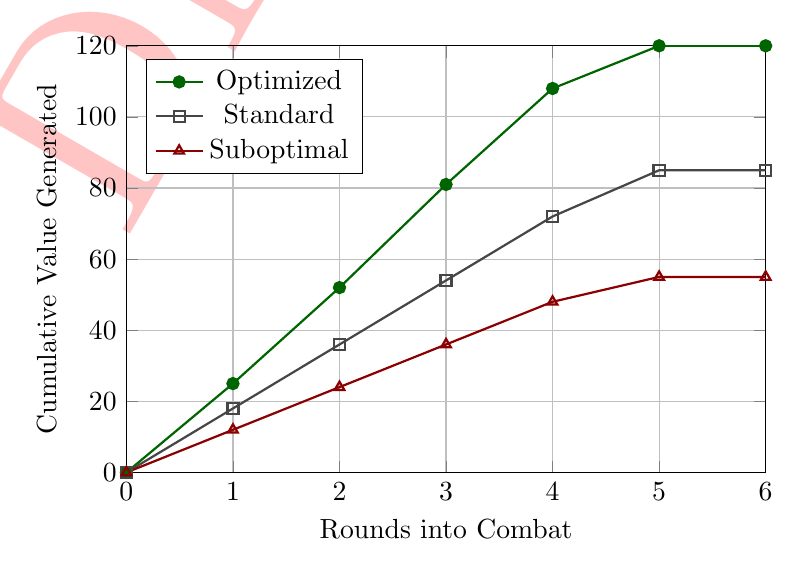
\begin{tikzpicture}
\begin{axis}[
    xlabel={Rounds into Combat},
    ylabel={Cumulative Value Generated},
    xmin=0, xmax=6,
    ymin=0, ymax=120,
    legend pos=north west,
    grid=major,
    width=0.8\textwidth,
    height=7cm
]
% Optimized action economy
\addplot[color=dragongreen,thick,mark=*] coordinates {
    (0,0) (1,25) (2,52) (3,81) (4,108) (5,120) (6,120)
};
\addlegendentry{Optimized}

% Standard action economy
\addplot[color=shadowgray,thick,mark=square] coordinates {
    (0,0) (1,18) (2,36) (3,54) (4,72) (5,85) (6,85)
};
\addlegendentry{Standard}

% Poor action economy
\addplot[color=bloodred,thick,mark=triangle] coordinates {
    (0,0) (1,12) (2,24) (3,36) (4,48) (5,55) (6,55)
};
\addlegendentry{Suboptimal}
\end{axis}
\end{tikzpicture}
\caption{Cumulative Value by Action Economy Efficiency}
\end{figure}

\section{Reaction Timing Probabilities}

\subsection{Opportunity Attack Frequency}

Given $n$ enemies and movement patterns:
\begin{equation}
P(\text{OA per round}) = 1 - (1 - p_{\text{move}})^n
\end{equation}

Where $p_{\text{move}} \approx 0.3$ for typical encounters.

\subsection{Counterspell Decision Trees}

Optimal counterspell usage against spell of level $L$:
\begin{equation}
\text{Counter if: } P(\text{success}) \times V(\text{prevented}) > V(\text{slot}_3)
\end{equation}

For upcast counterspell:
\begin{equation}
P(\text{success}) = \begin{cases}
1.0 & \text{if } L \leq \text{slot level} \\
0.5 + 0.05 \times \text{modifier} & \text{if } L > \text{slot level}
\end{cases}
\end{equation}

\chapter{Long-Term Resource Management}

\firstletter{S}urvival through an adventuring day requires careful husbandry of limited resources.

\section{The Adventuring Day Budget}

Standard adventuring day expectations:
\begin{itemize}
    \item 6-8 medium encounters
    \item 2 short rests
    \item Resource expenditure: 75\% of daily total
\end{itemize}

\subsection{Spell Slot Economy}

Optimal spell slot distribution across $E$ encounters:
\begin{equation}
\text{Slots per encounter} = \frac{\text{Total Slots} \times 0.75}{E}
\end{equation}

\begin{table}[h]
\centering
\begin{tabular}{@{}lcccc@{}}
\toprule
\textbf{Caster Level} & \textbf{Total Slots} & \textbf{Per Encounter (6E)} & \textbf{Per Encounter (8E)} \\
\midrule
5 & 9 & 1.1 & 0.8 \\
10 & 15 & 1.9 & 1.4 \\
15 & 19 & 2.4 & 1.8 \\
20 & 22 & 2.8 & 2.1 \\
\bottomrule
\end{tabular}
\caption{Spell Slot Budget by Encounter Frequency}
\end{table}

\section{Hit Dice Recovery Optimization}

\subsection{Expected Healing Per Die}

For a d$X$ hit die with Constitution modifier $m$:
\begin{equation}
E[\text{healing}] = \frac{X+1}{2} + m
\end{equation}

\subsection{Short Rest Efficiency}

Optimal hit dice usage threshold:
\begin{equation}
\text{Use HD if: } \text{Current HP} < \text{Max HP} \times \left(0.6 - 0.05 \times \text{remaining encounters}\right)
\end{equation}

\begin{figure}[h]
\centering
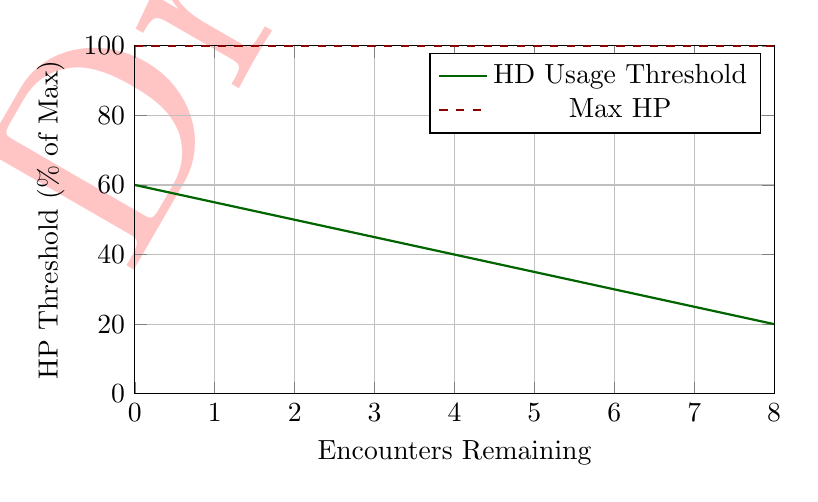
\begin{tikzpicture}
\begin{axis}[
    xlabel={Encounters Remaining},
    ylabel={HP Threshold (\% of Max)},
    xmin=0, xmax=8,
    ymin=0, ymax=100,
    grid=major,
    width=0.8\textwidth,
    height=6cm
]
\addplot[color=dragongreen,thick,domain=0:8] {60 - 5*x};
\addplot[color=bloodred,dashed,thick] coordinates {(0,100) (8,100)};
\addlegendentry{HD Usage Threshold}
\addlegendentry{Max HP}
\end{axis}
\end{tikzpicture}
\caption{Optimal Hit Dice Usage Thresholds}
\end{figure}

\section{Consumable Resource Valuation}

\subsection{Potion Economy}

Expected value of healing potion:
\begin{equation}
V(\text{potion}) = P(\text{prevents KO}) \times V(\text{actions saved}) + E[\text{healing}]
\end{equation}

Break-even point for potion usage:
\begin{equation}
\text{Gold cost} = \text{Expected party damage prevented} \times \text{Gold per HP}
\end{equation}

\chapter{Multiclassing Mathematics}

\firstletter{T}he art of combining classes requires precise understanding of power progression breakpoints.

\section{Level Progression Analysis}

\subsection{Power Spike Identification}

Character power as function of levels:
\begin{equation}
P(L_1, L_2, ..., L_n) = \sum_{i=1}^{n} f_i(L_i) + \text{Synergy}(L_1, ..., L_n)
\end{equation}

\begin{figure}[h]
\centering
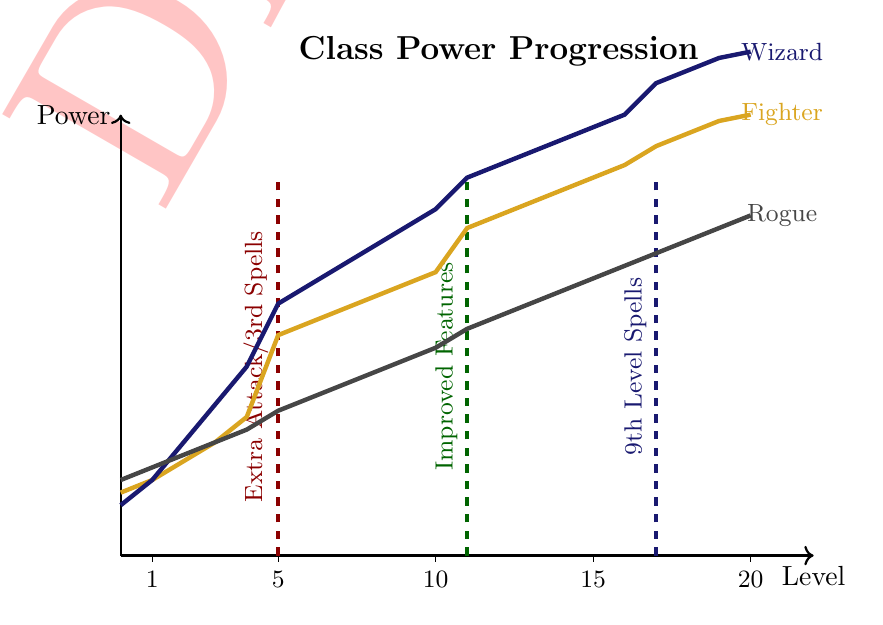
\begin{tikzpicture}[scale=0.8]
    % Title
    \node[font=\large\bfseries] at (6,8) {Class Power Progression};
    
    % Axes
    \draw[thick, ->] (0,0) -- (11,0) node[anchor=north] {Level};
    \draw[thick, ->] (0,0) -- (0,7) node[anchor=east] {Power};
    
    % Level marks
    \foreach \x in {1,5,10,15,20} {
        \draw (\x/2,0) -- (\x/2,-0.1) node[below] {\small\x};
    }
    
    % Power spike indicators
    \draw[bloodred, ultra thick, dashed] (2.5,0) -- (2.5,6);
    \node[bloodred, rotate=90, anchor=south] at (2.5,3) {\small Extra Attack/3rd Spells};
    
    \draw[dragongreen, ultra thick, dashed] (5.5,0) -- (5.5,6);
    \node[dragongreen, rotate=90, anchor=south] at (5.5,3) {\small Improved Features};
    
    \draw[mysticblue, ultra thick, dashed] (8.5,0) -- (8.5,6);
    \node[mysticblue, rotate=90, anchor=south] at (8.5,3) {\small 9th Level Spells};
    
    % Class progression lines
    % Fighter
    \draw[goldink, ultra thick] plot coordinates {
        (0,1) (0.5,1.2) (1,1.5) (1.5,1.8) (2,2.2) (2.5,3.5) % Level 5 spike
        (3,3.7) (3.5,3.9) (4,4.1) (4.5,4.3) (5,4.5) (5.5,5.2) % Level 11 spike
        (6,5.4) (6.5,5.6) (7,5.8) (7.5,6) (8,6.2) (8.5,6.5) % Level 17
        (9,6.7) (9.5,6.9) (10,7)
    };
    \node[goldink, font=\small] at (10.5,7) {Fighter};
    
    % Wizard
    \draw[mysticblue, ultra thick] plot coordinates {
        (0,0.8) (0.5,1.2) (1,1.8) (1.5,2.4) (2,3) (2.5,4) % Level 5 spike
        (3,4.3) (3.5,4.6) (4,4.9) (4.5,5.2) (5,5.5) (5.5,6) % Level 11 spike
        (6,6.2) (6.5,6.4) (7,6.6) (7.5,6.8) (8,7) (8.5,7.5) % Level 17 spike
        (9,7.7) (9.5,7.9) (10,8)
    };
    \node[mysticblue, font=\small] at (10.5,8) {Wizard};
    
    % Rogue
    \draw[shadowgray, ultra thick] plot coordinates {
        (0,1.2) (0.5,1.4) (1,1.6) (1.5,1.8) (2,2) (2.5,2.3) % Modest at 5
        (3,2.5) (3.5,2.7) (4,2.9) (4.5,3.1) (5,3.3) (5.5,3.6) % Modest at 11
        (6,3.8) (6.5,4) (7,4.2) (7.5,4.4) (8,4.6) (8.5,4.8) % Modest at 17
        (9,5) (9.5,5.2) (10,5.4)
    };
    \node[shadowgray, font=\small] at (10.5,5.4) {Rogue};
\end{tikzpicture}
\caption{Power Progression: Major Breakpoints by Class}
\end{figure}

\subsection{DPR Optimization}

For martial multiclass combinations:
\begin{equation}
\text{DPR} = \text{Attacks} \times (P(\text{hit}) \times E[\text{damage}]) + \text{Bonus Features}
\end{equation}

\begin{table}[h]
\centering
\begin{tabular}{@{}lccc@{}}
\toprule
\textbf{Build} & \textbf{Level Split} & \textbf{DPR at 20} & \textbf{Peak Level} \\
\midrule
Pure Fighter & 20 & 45.5 & 20 \\
Fighter/Barbarian & 11/9 & 48.2 & 20 \\
Paladin/Sorcerer & 6/14 & 52.1 & 17 \\
Paladin/Warlock & 7/13 & 49.8 & 15 \\
Rogue/Fighter & 15/5 & 41.3 & 18 \\
\bottomrule
\end{tabular}
\caption{Common Multiclass DPR Analysis}
\end{table}

\section{Spellcasting Multiclass}

\subsection{Effective Caster Level}

For multiclass spellcasters:
\begin{equation}
\text{Spell Slots} = f\left(\sum_{i} w_i \times L_i\right)
\end{equation}

Where weights $w$:
\begin{itemize}
    \item Full casters: $w = 1.0$
    \item Half casters: $w = 0.5$
    \item Third casters: $w = 0.33$
\end{itemize}

\begin{figure}[h]
\centering
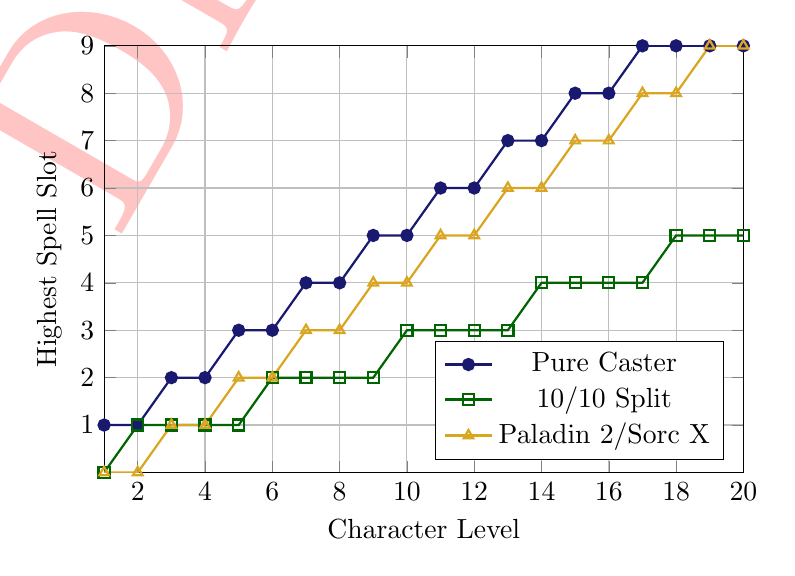
\begin{tikzpicture}
\begin{axis}[
    xlabel={Character Level},
    ylabel={Highest Spell Slot},
    xmin=1, xmax=20,
    ymin=0, ymax=9,
    ytick={1,2,3,4,5,6,7,8,9},
    legend pos=south east,
    grid=major,
    width=0.8\textwidth,
    height=7cm
]
% Pure caster
\addplot[color=mysticblue,thick,mark=*] coordinates {
    (1,1) (2,1) (3,2) (4,2) (5,3) (6,3) (7,4) (8,4) (9,5)
    (10,5) (11,6) (12,6) (13,7) (14,7) (15,8) (16,8) (17,9)
    (18,9) (19,9) (20,9)
};
\addlegendentry{Pure Caster}

% 10/10 split
\addplot[color=dragongreen,thick,mark=square] coordinates {
    (1,0) (2,1) (3,1) (4,1) (5,1) (6,2) (7,2) (8,2) (9,2)
    (10,3) (11,3) (12,3) (13,3) (14,4) (15,4) (16,4) (17,4)
    (18,5) (19,5) (20,5)
};
\addlegendentry{10/10 Split}

% Paladin 2/Sorcerer X
\addplot[color=goldink,thick,mark=triangle] coordinates {
    (1,0) (2,0) (3,1) (4,1) (5,2) (6,2) (7,3) (8,3) (9,4)
    (10,4) (11,5) (12,5) (13,6) (14,6) (15,7) (16,7) (17,8)
    (18,8) (19,9) (20,9)
};
\addlegendentry{Paladin 2/Sorc X}
\end{axis}
\end{tikzpicture}
\caption{Spell Slot Progression by Build}
\end{figure}

\section{Feat Selection Mathematics}

\subsection{ASI vs Feat Decision}

Expected value calculation:
\begin{equation}
V(\text{ASI}) = 2 \times \Delta\text{modifier} \times \text{uses per day}
\end{equation}

\begin{equation}
V(\text{Feat}) = \sum_{\text{benefits}} P(\text{trigger}) \times V(\text{effect})
\end{equation}

Common feat values:
\begin{itemize}
    \item \ability{Great Weapon Master}: +2.5 to +5 DPR
    \item \ability{Sharpshooter}: +3 to +6 DPR
    \item \ability{War Caster}: +15\% concentration saves
    \item \ability{Lucky}: $\approx$ +5\% success rate on critical rolls
\end{itemize}

\chapter{Magic Item Mathematics}

\firstletter{E}nchanted artifacts follow their own economic and mathematical principles.

\section{Item Rarity Distribution}

\subsection{Expected Items by Level}

Using standard treasure hoard tables:
\begin{equation}
E[\text{magic items}] = \sum_{\text{CR}} P(\text{hoard}) \times N(\text{items})
\end{equation}

\begin{table}[h]
\centering
\begin{tabular}{@{}lcccc@{}}
\toprule
\textbf{Party Level} & \textbf{Common} & \textbf{Uncommon} & \textbf{Rare} & \textbf{Very Rare} \\
\midrule
1-4 & 2-3 & 0-1 & 0 & 0 \\
5-10 & 4-6 & 3-5 & 1-2 & 0 \\
11-16 & 6-8 & 6-10 & 3-5 & 1-2 \\
17-20 & 8-10 & 10-15 & 6-10 & 3-5 \\
\bottomrule
\end{tabular}
\caption{Expected Cumulative Magic Items}
\end{table}

\section{Combat Rating Adjustment}

\subsection{Effective HP with Items}

For AC-boosting items:
\begin{equation}
\text{EHP} = \text{HP} \times \frac{20}{21 - (\text{enemy hit bonus} - \text{AC})}
\end{equation}

\subsection{Damage Output Scaling}

With +X weapons:
\begin{equation}
\Delta\text{DPR} = n \times \left(X + X \times P(\text{hit})\right)
\end{equation}

Where $n$ = number of attacks per round.

\begin{figure}[h]
\centering
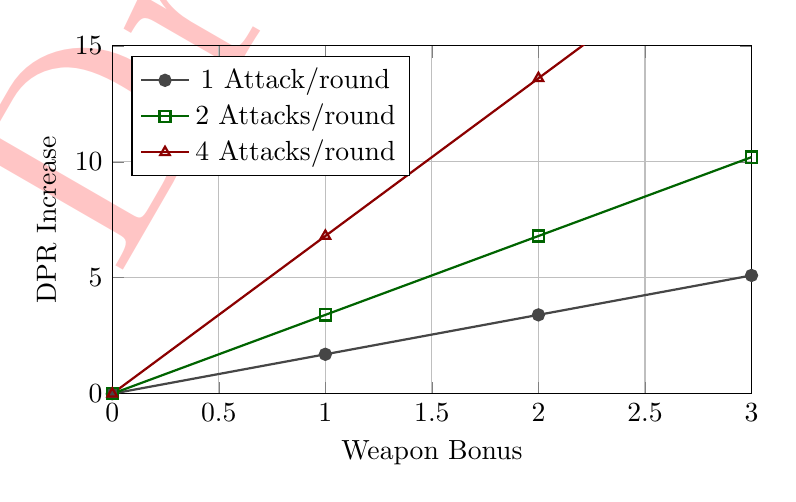
\begin{tikzpicture}
\begin{axis}[
    xlabel={Weapon Bonus},
    ylabel={DPR Increase},
    xmin=0, xmax=3,
    ymin=0, ymax=15,
    legend pos=north west,
    grid=major,
    width=0.8\textwidth,
    height=6cm
]
% 1 attack
\addplot[color=shadowgray,thick,mark=*] coordinates {
    (0,0) (1,1.7) (2,3.4) (3,5.1)
};
\addlegendentry{1 Attack/round}

% 2 attacks
\addplot[color=dragongreen,thick,mark=square] coordinates {
    (0,0) (1,3.4) (2,6.8) (3,10.2)
};
\addlegendentry{2 Attacks/round}

% 4 attacks
\addplot[color=bloodred,thick,mark=triangle] coordinates {
    (0,0) (1,6.8) (2,13.6) (3,20.4)
};
\addlegendentry{4 Attacks/round}
\end{axis}
\end{tikzpicture}
\caption{DPR Scaling with Magic Weapons}
\end{figure}

\section{Homebrew Item Balancing}

\subsection{Power Budget Formula}

For creating balanced magic items:
\begin{equation}
\text{Power Budget} = \text{Base by Rarity} + \sum(\text{Drawbacks}) - \sum(\text{Benefits})
\end{equation}

Rarity budgets:
\begin{itemize}
    \item Common: 1-2 points
    \item Uncommon: 3-5 points
    \item Rare: 6-10 points
    \item Very Rare: 11-17 points
    \item Legendary: 18-25 points
\end{itemize}

\chapter{Party Synergy Mathematics}

\firstletter{A}dventurers united multiply their effectiveness beyond simple addition.

\section{Role Coverage Optimization}

\subsection{Party Composition Matrix}

Optimal party coverage score:
\begin{equation}
S = \sum_{\text{roles}} \min(1, \text{Coverage}) \times \text{Weight}
\end{equation}

Essential roles and weights:
\begin{itemize}
    \item Tank/Frontline: $w = 0.25$
    \item Healing: $w = 0.20$
    \item Damage (single): $w = 0.20$
    \item Damage (AoE): $w = 0.15$
    \item Control: $w = 0.15$
    \item Utility: $w = 0.05$
\end{itemize}

\begin{table}[h]
\centering
\begin{tabular}{@{}lccccc@{}}
\toprule
\textbf{Composition} & \textbf{Tank} & \textbf{Heal} & \textbf{DPS} & \textbf{Control} & \textbf{Score} \\
\midrule
4 Strikers & 0.3 & 0.1 & 2.0 & 0.2 & 0.68 \\
Balanced & 1.0 & 0.8 & 1.2 & 0.8 & 0.94 \\
Tank Heavy & 2.0 & 0.6 & 0.6 & 0.4 & 0.82 \\
Control Focus & 0.5 & 0.7 & 0.8 & 1.5 & 0.88 \\
\bottomrule
\end{tabular}
\caption{Party Composition Effectiveness}
\end{table}

\section{Buff Stacking Mathematics}

\subsection{Multiplicative Benefits}

When buffs stack multiplicatively:
\begin{equation}
\text{Total Effectiveness} = \prod_{i=1}^{n} (1 + b_i)
\end{equation}

Common multiplicative buffs:
\begin{itemize}
    \item \spell{Bless}: +2.5 average to hit ($\approx$ +12.5\% hit rate)
    \item \spell{Haste}: ×2 attacks (with restrictions)
    \item Advantage: $\approx$ +5 effective bonus
    \item \ability{Bardic Inspiration}: +4.5 average
\end{itemize}

\begin{figure}[h]
\centering
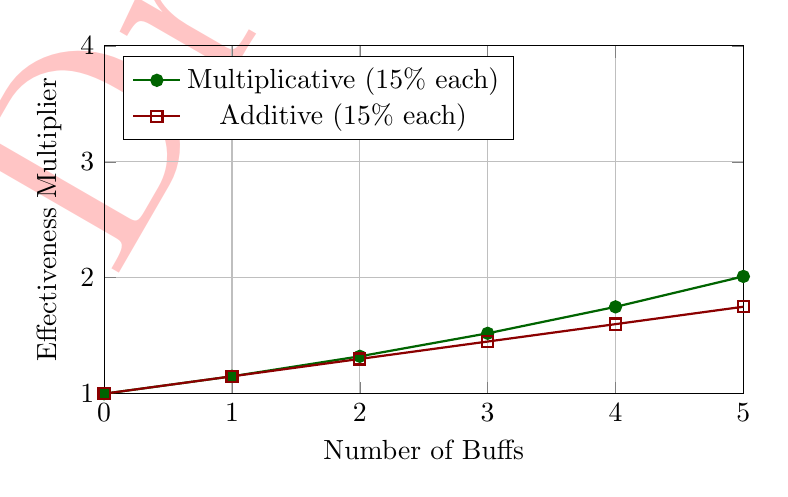
\begin{tikzpicture}
\begin{axis}[
    xlabel={Number of Buffs},
    ylabel={Effectiveness Multiplier},
    xmin=0, xmax=5,
    ymin=1, ymax=4,
    legend pos=north west,
    grid=major,
    width=0.8\textwidth,
    height=6cm
]
% Multiplicative stacking
\addplot[color=dragongreen,thick,mark=*,domain=0:5,samples=6] {1.15^x};
\addlegendentry{Multiplicative (15\% each)}

% Additive stacking
\addplot[color=bloodred,thick,mark=square,domain=0:5,samples=6] {1 + 0.15*x};
\addlegendentry{Additive (15\% each)}
\end{axis}
\end{tikzpicture}
\caption{Buff Stacking Methods Comparison}
\end{figure}

\section{Focus Fire Efficiency}

\subsection{Lanchester's Laws Application}

For focused targeting:
\begin{equation}
\text{Effective DPS} = \text{Party DPS} \times \sqrt{\frac{\text{Focus Factor}}{\text{Enemy Count}}}
\end{equation}

Time to eliminate threats:
\begin{equation}
t_{\text{focused}} = \frac{\sum \text{Enemy HP}}{\text{Party DPS}} \times \text{Overkill Factor}
\end{equation}

Where Overkill Factor $\approx 1.1$-$1.2$ for typical parties.

\chapter{Environmental Storytelling}

\firstletter{T}he world itself tells stories through weather, terrain, and the passage of time.

\section{Making Travel Matter}

\subsection{The Journey as Story}

Instead of "You travel for three days," consider:
\begin{itemize}
    \item \textbf{Day 1}: "Rain begins as you leave town. The merchant caravan you're following seems nervous."
    \item \textbf{Day 2}: "You find the caravan's remains. No bodies, but blood and strange tracks."
    \item \textbf{Day 3}: "The rain stops. In the sudden silence, you hear crying from the woods."
\end{itemize}

\subsection{Meaningful Random Encounters}

Roll not for "what attacks" but for "what story emerges":
\begin{itemize}
    \item \textbf{1-2}: Evidence of the main threat (tracks, victims, warnings)
    \item \textbf{3-4}: Local color (merchants, pilgrims, wanderers with news)
    \item \textbf{5}: Environmental challenge (bridge out, storm, blocked pass)
    \item \textbf{6}: Opportunity (lost treasure, helpful NPC, shortcut)
\end{itemize}

\begin{figure}[h]
\centering
\begin{tikzpicture}[scale=0.8]
    % Title
    \node[font=\large\bfseries] at (0,9) {Terrain Types and Travel};
    
    % Terrain hexes
    \foreach \terrain/\x/\y/\col/\dc/\enc/\speed in /1.0,%
        {Grassland}/3/5/dragongreen/10/{10\%}/1.0,%
        {Forest}/-3/5/{dragongreen!80!black}/15/{15\%}/0.75,%
        {Mountain}/0/3/{shadowgray!60}/15/{20\%}/0.5,%
        {Swamp}/3/2/{dragongreen!50!shadowgray}/15/{25\%}/0.5,%
        {Desert}/-3/2/goldink/20/{15\%}/0.75%
    } {
        % Hex shape
        \begin{scope}[shift={(\x,\y)}]
            \draw[\col, ultra thick, fill=\col!30] 
                (0:1) -- (60:1) -- (120:1) -- (180:1) -- (240:1) -- (300:1) -- cycle;
            
            % Terrain name
            \node[font=\small\bfseries] at (0,0.3) {\terrain};
            
            % Stats
            \node[font=\tiny] at (0,-0.1) {DC \dc};
            \node[font=\tiny] at (0,-0.4) {Enc: \enc};
            \node[font=\tiny] at (0,-0.7) {Speed: \speed};
        \end{scope}
    }
    
    % Legend
    \draw[thick] (-5,0) rectangle (5,-1.5);
    \node[font=\small\bfseries] at (0,-0.3) {Travel Modifiers};
    \node[font=\tiny, anchor=west] at (-4.5,-0.7) {DC: Navigation difficulty};
    \node[font=\tiny, anchor=west] at (-4.5,-1) {Enc: Random encounter chance/hour};
    \node[font=\tiny, anchor=west] at (-4.5,-1.3) {Speed: Movement rate multiplier};
\end{tikzpicture}
\caption{Terrain Travel Parameters: Choose Your Path Wisely}
\end{figure}

\section{Traps as Puzzles}

\subsection{Better Than "Roll to Not Die"}

Great traps telegraph danger and reward cleverness:
\begin{itemize}
    \item \textbf{Clue}: Scorched walls suggest fire
    \item \textbf{Pattern}: The safe path follows the moon mosaic
    \item \textbf{Solution}: Multiple approaches work
    \item \textbf{Failure}: Interesting, not instant death
\end{itemize}

\fantasyquote{"The best trap is one the players voluntarily walk into, knowing it's a trap, because the treasure is that tempting." —Grimtooth}

\subsection{Environmental Hazards}

Nature's traps need no dungeon:
\begin{itemize}
    \item \textbf{Avalanche}: Loud noises trigger, Dex save or buried
    \item \textbf{Quicksand}: Strength to escape, worse with struggling
    \item \textbf{Forest Fire}: Spreading doom, smoke and choices
    \item \textbf{Flash Flood}: Minutes of warning, test of priorities
\end{itemize}

\chapter{Social Encounter Mechanics}

\firstletter{W}ords can be as powerful as swords when wielded with mathematical precision.

\section{Skill Check Probabilities}

\subsection{Degrees of Success}

For social encounters with scaling DCs:
\begin{align}
\text{Critical Success} &: \text{Roll} \geq \text{DC} + 10 \\
\text{Success} &: \text{DC} \leq \text{Roll} < \text{DC} + 10 \\
\text{Failure} &: \text{DC} - 5 \leq \text{Roll} < \text{DC} \\
\text{Critical Failure} &: \text{Roll} < \text{DC} - 5
\end{align}

\subsection{Group Check Mathematics}

For group checks with $n$ participants:
\begin{equation}
P(\text{group success}) = P\left(\text{successes} \geq \lceil\frac{n}{2}\rceil\right)
\end{equation}

Using binomial distribution:
\begin{equation}
P = \sum_{k=\lceil n/2 \rceil}^{n} \binom{n}{k} p^k (1-p)^{n-k}
\end{equation}

\begin{figure}[h]
\centering
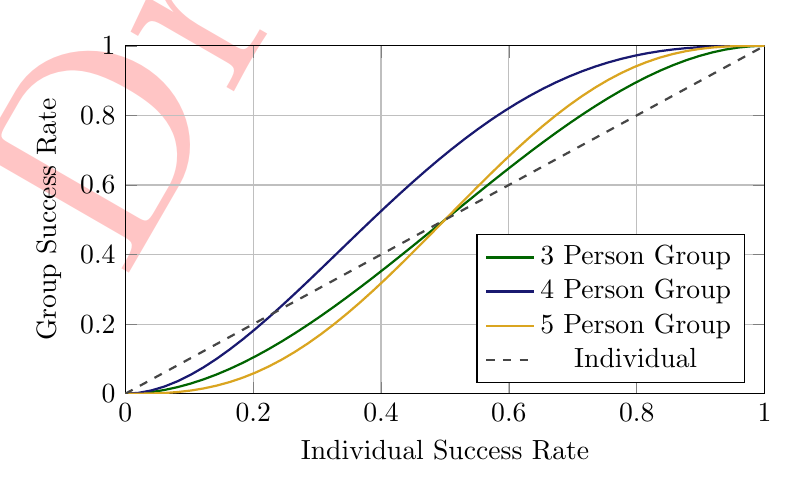
\begin{tikzpicture}
\begin{axis}[
    xlabel={Individual Success Rate},
    ylabel={Group Success Rate},
    xmin=0, xmax=1,
    ymin=0, ymax=1,
    legend pos=south east,
    grid=major,
    width=0.8\textwidth,
    height=6cm
]
% 3 person group
\addplot[color=dragongreen,thick,domain=0:1,samples=50] 
    {x^3 + 3*x^2*(1-x)};
\addlegendentry{3 Person Group}

% 4 person group
\addplot[color=mysticblue,thick,domain=0:1,samples=50] 
    {x^4 + 4*x^3*(1-x) + 6*x^2*(1-x)^2};
\addlegendentry{4 Person Group}

% 5 person group
\addplot[color=goldink,thick,domain=0:1,samples=50] 
    {x^5 + 5*x^4*(1-x) + 10*x^3*(1-x)^2};
\addlegendentry{5 Person Group}

% Individual (reference)
\addplot[color=shadowgray,dashed,thick,domain=0:1] {x};
\addlegendentry{Individual}
\end{axis}
\end{tikzpicture}
\caption{Group Check Success Rates}
\end{figure}

\chapter{Stealth and Perception}

\firstletter{S}hadows and sight follow predictable patterns for those who understand the mathematics.

\section{Stealth Chain Probabilities}

\subsection{Extended Stealth Sequences}

Probability of maintaining stealth over $n$ checks:
\begin{equation}
P(\text{remain hidden}) = \prod_{i=1}^{n} P(\text{success}_i)
\end{equation}

With consistent DC and modifier:
\begin{equation}
P = \left(\frac{21 - (\text{DC} - \text{modifier})}{20}\right)^n
\end{equation}

\subsection{Group Stealth Optimization}

Optimal formation with mixed stealth abilities:
\begin{itemize}
    \item Scouts: High stealth characters advance first
    \item Support: \spell{Pass Without Trace} (+10 to all)
    \item Spacing: Minimize group checks
\end{itemize}

Expected detection distance:
\begin{equation}
d_{\text{detection}} = \frac{\text{Base Range}}{1 + e^{-0.2(\text{Perception} - \text{Stealth})}}
\end{equation}

\chapter{Between Adventures}

\firstletter{N}ot all heroism happens in dungeons. The quiet moments between adventures shape characters as much as any dragon.

\section{Meaningful Downtime}

\subsection{Growing the Legend}

Downtime activities that build story:
\begin{itemize}
    \item \textbf{Carousing}: Make a contact, make an enemy, wake up married
    \item \textbf{Research}: Uncover the villain's weakness, find the lost temple
    \item \textbf{Crafting}: Not just items—relationships, reputation, rivalries
    \item \textbf{Training}: Learn from masters, teach students, found schools
\end{itemize}

\subsection{The Living World}

While heroes rest, the world moves:
\begin{itemize}
    \item Villains advance their plans
    \item Allies face their own challenges
    \item Political situations shift
    \item Opportunities expire
\end{itemize}

\fantasyquote{"I spent a month learning elvish. In that time, the necromancer raised an army. Worth it? Ask me in elvish." —Theodora the Linguist}

\subsection{Success Probability}

For complex items requiring checks:
\begin{equation}
P(\text{masterwork}) = P(\text{all checks succeed}) = p^n
\end{equation}

Where $n$ = number of required checks.

\begin{table}[h]
\centering
\begin{tabular}{@{}lccc@{}}
\toprule
\textbf{Item Rarity} & \textbf{Base DC} & \textbf{Time (days)} & \textbf{Cost Multiplier} \\
\midrule
Common & 10 & 4 & 0.5× \\
Uncommon & 12 & 20 & 0.5× \\
Rare & 15 & 100 & 0.5× \\
Very Rare & 18 & 500 & 0.5× \\
Legendary & 20 & 2500 & 0.5× \\
\bottomrule
\end{tabular}
\caption{Magic Item Crafting Requirements}
\end{table}

\section{Training Time Mathematics}

\subsection{Skill Development}

Learning curve for new proficiencies:
\begin{equation}
\text{Days Required} = \frac{250}{\text{Intelligence Modifier} + 1}
\end{equation}

Cost scaling:
\begin{equation}
\text{Total Cost} = 250 \times \text{Instructor Quality Multiplier}
\end{equation}

\chapter{Legendary Artifacts of Power}

\firstletter{T}hroughout history, certain items have transcended mere enchantment to become legends in their own right. These artifacts reshape the very mathematics of reality around them.

\section{The Codex of Infinite Spells}

\textit{Wondrous item, legendary (requires attunement)}

This massive tome contains every spell that has ever been conceived and many that have yet to be discovered. Its pages number exactly $\aleph_0$—a true mathematical infinity contained within finite binding.

\subsection{Properties}
\begin{itemize}
    \item The codex has 5d8 + 22 pages with spells
    \item Each page contains one spell, determined randomly
    \item Once per day, can turn to a new page (10\% chance of losing access to current page forever)
    \item Casting a spell from the codex requires no spell slots
\end{itemize}

\subsection{Mathematical Anomaly}
The codex violates normal spellcasting mathematics:
\begin{equation}
\text{Effective Caster Level} = \text{Reader Level} + 1d4
\end{equation}

\fantasyquote{"I have studied the Codex for forty years, and I have seen but a fraction of its first chapter." —Bigby}

\section{The Sword of Kas}

\textit{Weapon (longsword), artifact (requires attunement)}

Forged from the hatred of a betrayed lieutenant, this blade exists to destroy its creator—the lich Vecna. Its power grows with each undead slain.

\subsection{Cumulative Power}
\begin{equation}
\text{Attack Bonus} = +3 + \left\lfloor\frac{\text{Undead Slain}}{100}\right\rfloor \text{ (max +6)}
\end{equation}

\subsection{Vecna's Bane}
\begin{itemize}
    \item Against Vecna: +10 to hit, deals an extra 10d6 damage
    \item Against undead: Advantage on attacks, +2d6 radiant damage
    \item Sentient: Int 15, Wis 13, Cha 16, Chaotic Evil
    \item Weakness: 5\% chance per day to attempt domination of wielder
\end{itemize}

\section{The Deck of Many Things}

\textit{Wondrous item, legendary}

Perhaps no artifact better embodies the intersection of fate and mathematics than this infamous deck of cards. Each draw fundamentally alters probability itself.

\begin{table}[h]
\centering
\small
\begin{tabular}{@{}lcc@{}}
\toprule
\textbf{Card} & \textbf{Probability} & \textbf{Effect Summary} \\
\midrule
The Void & 4.5\% & Soul trapped in object \\
The Throne & 4.5\% & Gain a keep \\
The Fates & 4.5\% & Undo one event \\
The Gem & 4.5\% & Gain 50,000 gp jewelry \\
The Fool & 4.5\% & Lose 10,000 XP, draw again \\
The Ruin & 4.5\% & Lose all wealth \\
The Skull & 4.5\% & Fight avatar of death \\
\bottomrule
\end{tabular}
\caption{Sample Deck Probabilities (22-card deck)}
\end{table}

\chapter{Spellcraft: Theory and Practice}

\firstletter{T}he art of spellcasting bridges the gap between will and reality, between thought and manifestation. Each spell is a mathematical formula given life.

\section{Anatomy of a Spell}

Every spell consists of three fundamental components that must balance:

\begin{equation}
\text{Spell Power} = \frac{\text{Verbal} \times \text{Somatic} \times \text{Material}}{\text{Casting Time}}
\end{equation}

\begin{figure}[h]
\centering
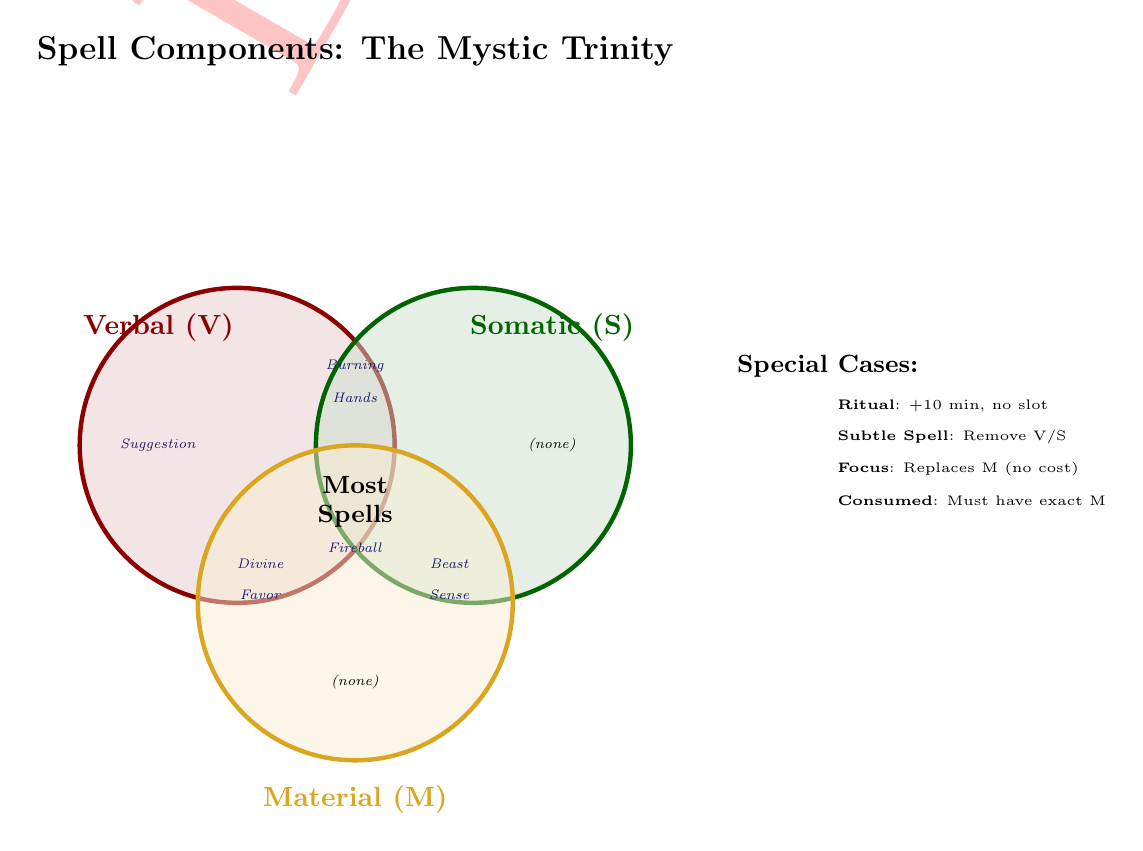
\begin{tikzpicture}[scale=1]
    % Title
    \node[font=\large\bfseries] at (0,6) {Spell Components: The Mystic Trinity};
    
    % Venn diagram of spell components
    % V circle
    \draw[bloodred, ultra thick, fill=bloodred!20, fill opacity=0.5] (-1.5,1) circle (2cm);
    \node[bloodred, font=\bfseries] at (-2.5,2.5) {Verbal (V)};
    
    % S circle
    \draw[dragongreen, ultra thick, fill=dragongreen!20, fill opacity=0.5] (1.5,1) circle (2cm);
    \node[dragongreen, font=\bfseries] at (2.5,2.5) {Somatic (S)};
    
    % M circle
    \draw[goldink, ultra thick, fill=goldink!20, fill opacity=0.5] (0,-1) circle (2cm);
    \node[goldink, font=\bfseries] at (0,-3.5) {Material (M)};
    
    % Example spells in regions
    \node[font=\tiny] at (-2.5,1) {\spell{Suggestion}};
    \node[font=\tiny] at (2.5,1) {\textit{(none)}};
    \node[font=\tiny] at (0,-2) {\textit{(none)}};
    
    % VS intersection
    \node[font=\tiny] at (0,2) {\spell{Burning}};
    \node[font=\tiny] at (0,1.6) {\spell{Hands}};
    
    % VM intersection
    \node[font=\tiny] at (-1.2,-0.5) {\spell{Divine}};
    \node[font=\tiny] at (-1.2,-0.9) {\spell{Favor}};
    
    % SM intersection
    \node[font=\tiny] at (1.2,-0.5) {\spell{Beast}};
    \node[font=\tiny] at (1.2,-0.9) {\spell{Sense}};
    
    % VSM center
    \node[font=\small\bfseries] at (0,0.5) {Most};
    \node[font=\small\bfseries] at (0,0.1) {Spells};
    \node[font=\tiny] at (0,-0.3) {\spell{Fireball}};
    
    % Special cases
    \begin{scope}[shift={(6,0)}]
        \node[font=\small\bfseries] at (0,2) {Special Cases:};
        \node[font=\tiny, anchor=west] at (0,1.5) {\textbf{Ritual}: +10 min, no slot};
        \node[font=\tiny, anchor=west] at (0,1.1) {\textbf{Subtle Spell}: Remove V/S};
        \node[font=\tiny, anchor=west] at (0,0.7) {\textbf{Focus}: Replaces M (no cost)};
        \node[font=\tiny, anchor=west] at (0,0.3) {\textbf{Consumed}: Must have exact M};
    \end{scope}
\end{tikzpicture}
\caption{The Component Trinity: What Makes Magic Work}
\end{figure}

\subsection{Example: Fireball}

\spell{Fireball}\\  
\textit{3rd-level evocation}

\begin{itemize}
    \item \textbf{Casting Time}: 1 action
    \item \textbf{Range}: 150 feet
    \item \textbf{Components}: V, S, M (tiny ball of bat guano and sulfur)
    \item \textbf{Duration}: Instantaneous
\end{itemize}

A bright streak flashes from your pointing finger to a point you choose within range, then blossoms with a low roar into an explosion of flame.

\textbf{Mathematics}: Each creature in a 20-foot radius must make a Dexterity save. Damage = 8d6 fire (average 28).

\textbf{Scaling}: Damage increases by 1d6 per slot level above 3rd:
\begin{equation}
\damage{Total Damage} = (5 + \text{Slot Level}) \times d6
\end{equation}

\subsection{Example: Counterspell}

\spell{Counterspell}\\  
\textit{3rd-level abjuration}

The ultimate expression of magical negation, this spell collapses the mathematical framework of another spell before it can manifest.

\textbf{Reaction Timing}: When you see a creature within 60 feet casting a spell.

\textbf{Success Calculation}:
\begin{itemize}
    \item Automatic success if target spell level $\leq$ counterspell slot level
    \item Otherwise: DC = 10 + spell level, ability check using spellcasting modifier
\end{itemize}

\chapter{The Dungeon Master's Laboratory}

\firstletter{B}ehind the screen lies the true magic—the art of creating worlds that feel alive, challenges that excite, and stories that endure.

\section{World Building by the Numbers}

\subsection{Settlement Generation}

Population follows a power law distribution:
\begin{equation}
P(\text{size} = n) = \frac{k}{n^{2.3}}
\end{equation}

This creates realistic distributions:
\begin{itemize}
    \item Many small villages (50-400 people)
    \item Fewer towns (400-5,000 people)  
    \item Rare cities (5,000-25,000 people)
    \item Legendary metropolises (25,000+ people)
\end{itemize}

\subsection{Economic Simulation}

A settlement's magical economy follows:
\begin{equation}
\text{Magic Items Available} = \log_{10}(\text{Population}) \times \text{Prosperity Factor}
\end{equation}

\begin{table}[h]
\centering
\begin{tabular}{@{}lccc@{}}
\toprule
\textbf{Settlement} & \textbf{Base Item Limit} & \textbf{Spell Services} & \textbf{Magic Shops} \\
\midrule
Village & 50 gp & 1st level & None \\
Town & 200 gp & 3rd level & General goods \\
City & 1,000 gp & 5th level & Specialized \\
Metropolis & 10,000 gp & 9th level & Anything \\
\bottomrule
\end{tabular}
\caption{Settlement Magic Availability}
\end{table}

\section{Creating Memorable Villains}

\subsection{The Villain Power Curve}

A compelling villain should always be approximately:
\begin{equation}
\text{Villain CR} = \text{Average Party Level} + 2 + \frac{\text{Number of Minions}}{4}
\end{equation}

\subsection{Villain Action Economy}

Legendary villains break normal action economy rules:

\begin{figure}[h]
\centering
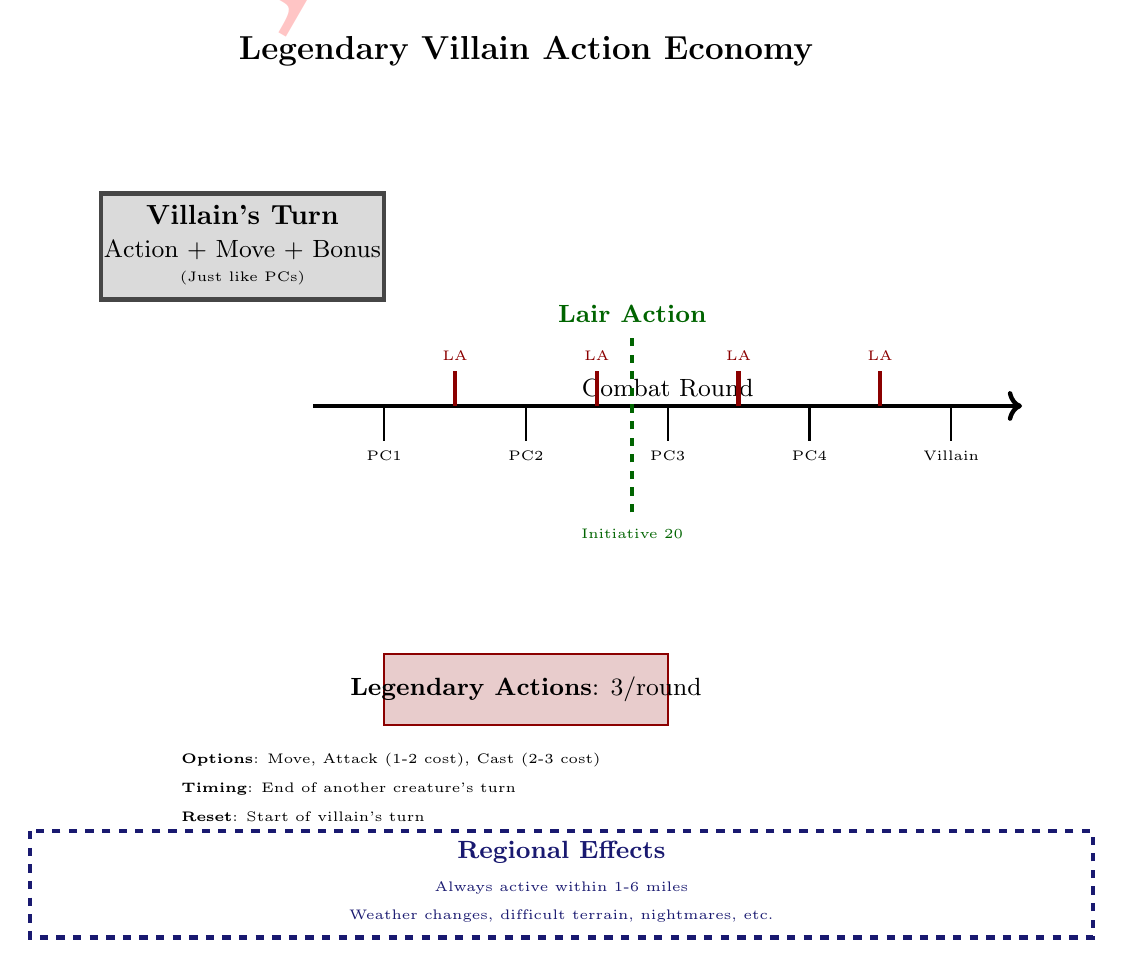
\begin{tikzpicture}[scale=0.9]
    % Title
    \node[font=\large\bfseries] at (0,8) {Legendary Villain Action Economy};
    
    % Regular turn
    \draw[shadowgray, ultra thick, fill=shadowgray!20] (-6,6) rectangle (-2,4.5);
    \node[font=\bfseries] at (-4,5.7) {Villain's Turn};
    \node[font=\small] at (-4,5.2) {Action + Move + Bonus};
    \node[font=\tiny] at (-4,4.8) {(Just like PCs)};
    
    % Legendary actions timeline
    \draw[ultra thick, ->] (-3,3) -- (7,3);
    \node[above, font=\small] at (2,3) {Combat Round};
    
    % PC turns
    \foreach \x/\name in {-2/PC1, 0/PC2, 2/PC3, 4/PC4, 6/Villain} {
        \draw[thick] (\x,3) -- (\x,2.5);
        \node[below, font=\tiny] at (\x,2.5) {\name};
    }
    
    % Legendary action markers
    \foreach \x in {-1, 1, 3, 5} {
        \draw[bloodred, ultra thick] (\x,3) -- (\x,3.5);
        \node[bloodred, above, font=\tiny] at (\x,3.5) {LA};
    }
    
    % Lair action
    \draw[dragongreen, ultra thick, dashed] (1.5,1.5) -- (1.5,4);
    \node[dragongreen, font=\small\bfseries] at (1.5,4.3) {Lair Action};
    \node[dragongreen, font=\tiny] at (1.5,1.2) {Initiative 20};
    
    % Legend boxes
    \begin{scope}[shift={(0,-1)}]
        \draw[bloodred, thick, fill=bloodred!20] (-2,-0.5) rectangle (2,0.5);
        \node[font=\small] at (0,0) {\textbf{Legendary Actions}: 3/round};
        
        \node[font=\tiny, anchor=west] at (-5,-1) {\textbf{Options}: Move, Attack (1-2 cost), Cast (2-3 cost)};
        \node[font=\tiny, anchor=west] at (-5,-1.4) {\textbf{Timing}: End of another creature's turn};
        \node[font=\tiny, anchor=west] at (-5,-1.8) {\textbf{Reset}: Start of villain's turn};
    \end{scope}
    
    % Regional effects
    \draw[mysticblue, ultra thick, dashed] (-7,-3) rectangle (8,-4.5);
    \node[mysticblue, font=\small\bfseries] at (0.5,-3.3) {Regional Effects};
    \node[mysticblue, font=\tiny] at (0.5,-3.8) {Always active within 1-6 miles};
    \node[mysticblue, font=\tiny] at (0.5,-4.2) {Weather changes, difficult terrain, nightmares, etc.};
\end{tikzpicture}
\caption{How Legendary Villains Cheat the Action Economy}
\end{figure}

\chapter{Running the Game}

\lettrine[lines=3]{B}{ehind} the screen, you are part storyteller, part referee, part improvisational actor, and part quantum physicist managing infinite possibilities.

\section{The First Rule}

The only rule that matters: \textbf{Is everyone having fun?}

All the mathematics, all the mechanics, all the carefully balanced encounters mean nothing if your players aren't engaged. Sometimes that means:
\begin{itemize}
    \item Letting the absurd plan work (with complications)
    \item Fudging a roll to avoid anticlimactic death
    \item Throwing out prepared content when players go off-script
    \item Saying "yes, and..." instead of "no, but..."
\end{itemize}

\section{The Art of Improvisation}

\subsection{The Random NPC Generator}

When players talk to that guard you never named:
\begin{enumerate}
    \item \textbf{Desire}: What do they want right now?
    \item \textbf{Fear}: What keeps them awake at night?
    \item \textbf{Quirk}: One memorable trait
    \item \textbf{Connection}: How they relate to the plot (even tangentially)
\end{enumerate}

\fantasyquote{"My players spent three hours planning to infiltrate the castle. They could have just asked—the guards were hiring." —Anonymous DM}

\section{Building Better Encounters}

\subsection{Beyond Hit Points}

Memorable encounters have:
\begin{itemize}
    \item \textbf{Terrain}: Height, cover, hazards, movement challenges
    \item \textbf{Objectives}: Beyond "kill everything"
    \item \textbf{Timers}: Rising water, ritual completion, reinforcements
    \item \textbf{Choices}: Save the hostage or stop the villain?
\end{itemize}

\subsection{The Villain's Escape Plan}

Smart villains always have:
\begin{itemize}
    \item \spell{Dimension Door} or \spell{Misty Step} prepared
    \item Loyal minions who take the fall
    \item Secret passages only they know
    \item Contingency spells for when things go wrong
    \item A reason to escape (revenge is a powerful motivator)
\end{itemize}

\chapter{Campaign Seeds and Sparks}

\lettrine[lines=3]{E}{very} great campaign begins with a simple question: "What if?"

\section{The Evolving World}

Your world should react to the party's actions:
\begin{itemize}
    \item That bandit camp they cleared? Now it's a goblin warren
    \item The noble they saved? She remembers, and has influence
    \item The artifact they sold? It's in the wrong hands now
    \item The villain they spared? He learned from his mistakes
\end{itemize}

\section{Adventure Hooks That Work}

\subsection{The Personal Hook}
"A letter arrives, water-stained and barely legible. It's from your sister—the one who disappeared ten years ago."

\subsection{The Ticking Clock}
"In three days, the stars align. If the cult completes their ritual then, the sealed god awakens. The nearest help is a week away."

\subsection{The Moral Dilemma}
"The dragon offers a deal: She'll stop raiding the countryside if the town delivers one person each month. The mayor is considering it."

\subsection{The Mystery}
"People in town are losing memories. First, they forget names. Then faces. Then everything. The clerics are baffled—divine magic isn't helping."

\section{Campaign Themes}

\begin{table}[h]
\centering
\begin{tabular}{@{}lll@{}}
\toprule
\textbf{Theme} & \textbf{Core Question} & \textbf{Mechanical Focus} \\
\midrule
Survival & Can we make it? & Resource management \\
Mystery & What's really happening? & Investigation skills \\
War & Which side wins? & Mass combat \\
Heist & Can we pull it off? & Planning and execution \\
Horror & What's the cost? & Sanity and corruption \\
Political & Who can we trust? & Social encounters \\
\bottomrule
\end{tabular}
\caption{Campaign Themes and Their Expression}
\end{table}

\chapter{Denizens of the Realms}

\lettrine[lines=3]{T}{he} world teems with life, from the humblest farmer to the mightiest dragon. Here are those who might aid or hinder your journey.

\section{Memorable NPCs}

\subsection{Gareth the Honest Merchant}
\textit{Human trader, lawful neutral}

"I deal in three currencies: gold, information, and favors. The exchange rate varies."

\begin{itemize}
    \item \textbf{Appearance}: Meticulously groomed, one gold tooth
    \item \textbf{Personality}: Scrupulously fair, annoyingly literal
    \item \textbf{Secret}: Retired spy, maintains old contacts
    \item \textbf{Useful For}: Equipment, rumors, introductions
\end{itemize}

\subsection{Lady Morwyn the Twice-Cursed}
\textit{Elf archmage, chaotic neutral}

"My first curse was immortality. My second was caring about mortals."

\begin{itemize}
    \item \textbf{Appearance}: Young-seeming, ancient eyes, silver hair
    \item \textbf{Personality}: Helpful but cryptic, easily bored
    \item \textbf{Secret}: Knows the location of three lost artifacts
    \item \textbf{Useful For}: Magical knowledge, planar travel, ancient history
\end{itemize}

\subsection{Brick the Philosophical}
\textit{Half-orc barbarian sage, neutral good}

"Violence is a question. The answer is usually 'yes,' but it's important to ask."

\begin{itemize}
    \item \textbf{Appearance}: Scarred, carries books and battleaxe equally
    \item \textbf{Personality}: Thoughtful, protective, unexpected wisdom
    \item \textbf{Secret}: Writes poetry, quite good actually
    \item \textbf{Useful For}: Muscle, surprising insights, mediating disputes
\end{itemize}

\chapter{Tales from the Table}

\lettrine[lines=3]{E}{very} calculation, every formula, every probability ultimately serves one purpose: creating unforgettable stories. Here are mathematical principles illustrated through actual play.

\section{The Paradox of the Peasant Railgun}

A famous thought experiment illustrates why physics and game mechanics must remain separate:

\textit{"If 2,000 peasants stand in a line and ready actions to pass a spear down the line, the spear travels 10,000 feet in 6 seconds—achieving a velocity of 1,136 mph."}

\textbf{The Mathematical Reality}: The spear still only deals 1d6 damage. Game mechanics model outcomes, not physics.

\section{The Lucky Halfling Theorem}

Consider Tilda Tosscobble, a halfling diviner with the Lucky feat:
\begin{itemize}
    \item Halfling Lucky: Reroll natural 1s
    \item Lucky feat: 3 rerolls per day
    \item Portent: Replace 2 rolls per day
    \item Advantage from various sources
\end{itemize}

Probability of failing a crucial roll:
\begin{equation}
P(\text{failure}) < 0.01\%
\end{equation}

\fantasyquote{"I don't believe in luck. I believe in being a halfling." —Tilda Tosscobble}

\chapter*{Appendix A: Quick Reference Tables}

\section*{Status Conditions}

\begin{figure}[h]
\centering
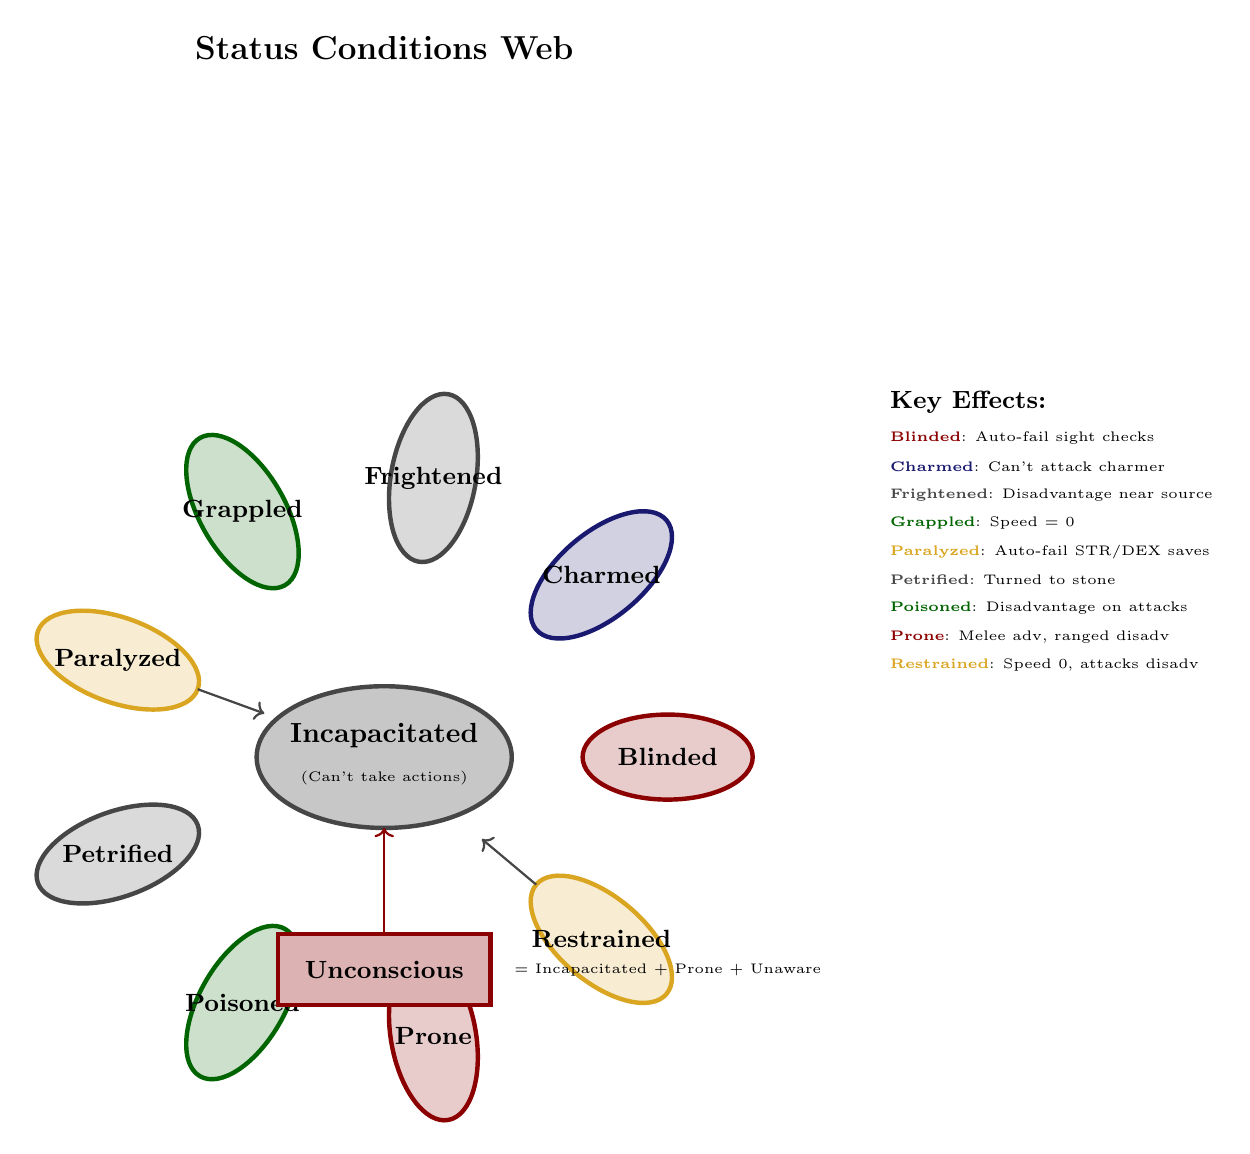
\begin{tikzpicture}[scale=0.9]
    % Title
    \node[font=\large\bfseries] at (0,10) {Status Conditions Web};
    
    % Define condition nodes in a circle
    \def\conditions{{
        {Blinded/0/bloodred},
        {Charmed/30/enchcolor}, 
        {Frightened/60/shadowgray},
        {Grappled/90/dragongreen},
        {Paralyzed/120/goldink},
        {Petrified/150/shadowgray},
        {Poisoned/180/dragongreen},
        {Prone/210/bloodred},
        {Restrained/240/goldink},
        {Stunned/270/mysticblue},
        {Unconscious/300/bloodred},
        {Incapacitated/330/shadowgray}
    }}
    
    % Draw condition nodes
    \foreach \cond/\angle/\col in {%
        {Blinded/0/bloodred},
        {Charmed/40/mysticblue}, 
        {Frightened/80/shadowgray},
        {Grappled/120/dragongreen},
        {Paralyzed/160/goldink},
        {Petrified/200/shadowgray},
        {Poisoned/240/dragongreen},
        {Prone/280/bloodred},
        {Restrained/320/goldink}%
    } {
        \begin{scope}[rotate=\angle]
            \draw[\col, ultra thick, fill=\col!20] (4,0) ellipse (1.2cm and 0.6cm);
            \node[font=\small\bfseries] at (4,0) {\cond};
        \end{scope}
    }
    
    % Central hub conditions
    \draw[shadowgray, ultra thick, fill=shadowgray!30] (0,0) ellipse (1.8cm and 1cm);
    \node[font=\bfseries] at (0,0.3) {Incapacitated};
    \node[font=\tiny] at (0,-0.3) {(Can't take actions)};
    
    % Draw connections showing which conditions include incapacitated
    \foreach \angle in {160, 320} { % Paralyzed, Stunned
        \draw[thick, shadowgray, ->] (\angle:2.8cm) -- (\angle:1.8cm);
    }
    
    % Unconscious special case
    \begin{scope}[shift={(0,-3)}]
        \draw[bloodred, ultra thick, fill=bloodred!30] (-1.5,-0.5) rectangle (1.5,0.5);
        \node[font=\small\bfseries] at (0,0) {Unconscious};
        \draw[thick, bloodred, ->] (0,0.5) -- (0,2);
        \node[font=\tiny, anchor=west] at (1.7,0) {= Incapacitated + Prone + Unaware};
    \end{scope}
    
    % Effect descriptions
    \begin{scope}[shift={(7,5)}]
        \node[anchor=west, font=\small\bfseries] at (0,0) {Key Effects:};
        \node[anchor=west, font=\tiny] at (0,-0.5) {\textcolor{bloodred}{\textbf{Blinded}}: Auto-fail sight checks};
        \node[anchor=west, font=\tiny] at (0,-0.9) {\textcolor{mysticblue}{\textbf{Charmed}}: Can't attack charmer};
        \node[anchor=west, font=\tiny] at (0,-1.3) {\textcolor{shadowgray}{\textbf{Frightened}}: Disadvantage near source};
        \node[anchor=west, font=\tiny] at (0,-1.7) {\textcolor{dragongreen}{\textbf{Grappled}}: Speed = 0};
        \node[anchor=west, font=\tiny] at (0,-2.1) {\textcolor{goldink}{\textbf{Paralyzed}}: Auto-fail STR/DEX saves};
        \node[anchor=west, font=\tiny] at (0,-2.5) {\textcolor{shadowgray}{\textbf{Petrified}}: Turned to stone};
        \node[anchor=west, font=\tiny] at (0,-2.9) {\textcolor{dragongreen}{\textbf{Poisoned}}: Disadvantage on attacks};
        \node[anchor=west, font=\tiny] at (0,-3.3) {\textcolor{bloodred}{\textbf{Prone}}: Melee adv, ranged disadv};
        \node[anchor=west, font=\tiny] at (0,-3.7) {\textcolor{goldink}{\textbf{Restrained}}: Speed 0, attacks disadv};
    \end{scope}
\end{tikzpicture}
\caption{Status Conditions and Their Relationships}
\end{figure}

\chapter*{Appendix B: The Mathematics of Dragons}

\section*{Age Categories and Power Scaling}

Dragons follow predictable growth patterns:

\begin{figure}[h]
\centering
\begin{tikzpicture}[scale=0.8]
    % Title
    \node[font=\large\bfseries] at (6,8) {The Draconic Life Cycle};
    
    % Draw dragon silhouettes of increasing size
    \foreach \stage/\x/\size/\col/\cr/\breath in {
        {Wyrmling}/0/1/{bloodred!50}/{2-4}/{2d8},
        {Young}/4/1.5/{bloodred!60}/{6-10}/{6d8},
        {Adult}/8/2.5/{bloodred!80}/{13-17}/{12d8},
        {Ancient}/12/3.5/{bloodred}/{20-24}/{18d8}%
    } {
        \begin{scope}[shift={(\x,0)}]
            % Dragon body (simplified)
            \draw[\col, ultra thick, fill=\col!30] (0,0) ellipse (\size cm and \size*0.6 cm);
            
            % Wings
            \draw[\col, thick, fill=\col!20] 
                (-\size*0.8,\size*0.3) .. controls (-\size*1.5,\size) and (-\size*1.2,\size*0.8) .. (-\size*0.8,\size*0.3);
            \draw[\col, thick, fill=\col!20] 
                (\size*0.8,\size*0.3) .. controls (\size*1.5,\size) and (\size*1.2,\size*0.8) .. (\size*0.8,\size*0.3);
            
            % Head
            \draw[\col, thick, fill=\col!40] (\size*0.8,\size*0.2) circle (\size*0.3 cm);
            
            % Label
            \node[font=\bfseries] at (0,-\size*0.8-0.5) {\stage};
            \node[font=\small] at (0,-\size*0.8-1) {CR \cr};
            \node[font=\tiny] at (0,-\size*0.8-1.4) {Breath: \breath};
        \end{scope}
    }
    
    % Power progression arrow
    \draw[ultra thick, ->, goldink] (0,-3) -- (12,-3);
    \node[goldink, font=\small] at (6,-3.5) {Age and Power};
    
    % Lair indicator
    \node[font=\small\itshape] at (10,-4.5) {Lair actions begin at Adult stage};
\end{tikzpicture}
\caption{Dragon Statistics by Age: From Hatchling to Ancient Terror}
\end{figure}

\chapter{Legendary Campaigns}

\lettrine[lines=3]{S}{ome} campaigns transcend mere adventure to become legend. These are their stories and lessons.

\section{The Tomb of Horrors Survivors}

\fantasyquote{"We entered as six confident heroes. Three emerged, forever changed. The halfling still won't go near green devil faces." —Robilar}

Lessons from the Tomb:
\begin{itemize}
    \item Paranoia is a survival trait
    \item 10-foot poles are worth their weight in platinum
    \item Sometimes retreat is victory
    \item The DM isn't trying to kill you; Acererak is
\end{itemize}

\section{The Rise of Tiamat Prevention Society}

A campaign where the heroes failed—and that made it legendary:
\begin{itemize}
    \item Tiamat rose despite their efforts
    \item The campaign continued in a dragon-ruled world
    \item Resistance movements, guerrilla warfare, small victories
    \item Players learned: failure creates better stories than success
\end{itemize}

\section{The Deck That Broke Everything}

One campaign. One Deck of Many Things. Chaos:
\begin{itemize}
    \item The fighter drew Throne and became a queen
    \item The wizard drew Void and spent six months being rescued
    \item The rogue drew Gem five times (cheating was involved)
    \item The cleric drew Balance and became chaotic evil
    \item Campaign pivoted to inter-party political drama
\end{itemize}

\fantasyquote{"We don't talk about the Deck Campaign. We also don't stop talking about it." —Anonymous}

\section{Creating Your Legend}

\subsection{Elements of Memorable Campaigns}

\begin{enumerate}
    \item \textbf{Stakes That Matter}: Not just the world—their world
    \item \textbf{Villains with Faces}: Enemies they love to hate
    \item \textbf{Consequences That Stick}: Actions echo through time
    \item \textbf{Moments of Choice}: When there's no right answer
    \item \textbf{Personal Investment}: NPCs they'd die for
\end{enumerate}

\subsection{The Perfect Final Session}

How legendary campaigns end:
\begin{itemize}
    \item Call back to the first session
    \item Each character gets their moment
    \item The impossible becomes possible
    \item Win or lose, it feels complete
    \item Leave one thread hanging (for dreams)
\end{itemize}

\section{Words of Wisdom}

From DMs who've run thousand-session campaigns:

\textbf{Gary the Ancient}: "The rules are guidelines. The story is law."

\textbf{Matt the Merciful}: "Kill characters, not players' enthusiasm."

\textbf{Diana the Dramatic}: "When in doubt, make it someone's backstory problem."

\textbf{Chris the Chronicler}: "Take notes. In ten years, you'll treasure them."

\textbf{Pat the Patient}: "The best campaigns grow like gardens, not blueprints."

\chapter*{Epilogue}

\lettrine[lines=3]{A}{s} we close this tome, remember that all the mathematics, all the probabilities, all the carefully balanced mechanics serve but one master: the shared story at your table.

The dice will betray you. A critical failure at the worst moment. A natural 20 when facing a lowly goblin. These are not flaws in the system—they are its greatest features. For in that unpredictability lies the spark that transforms a game into a legend.

\fantasyquote{"I have foreseen ten thousand futures. In none of them did the barbarian attempt to seduce the dragon. And yet here we are." —Nostradamus the Perpetually Surprised}

\section*{The Final Calculation}

If we must reduce the entirety of this game to a single equation, let it be this:

\begin{equation}
\text{Fun} = \frac{\text{Good Company} \times \text{Imagination}}{\text{Rules Arguments}}
\end{equation}

Use the mathematics in this codex not as chains but as wings. Let them lift your game to new heights while never forgetting that the best moments often come when you set the dice aside and simply ask, "What would your character do?"

\section*{Parting Wisdom}

\begin{itemize}
    \item The DM is not your enemy; probability is
    \item The only hit point that matters is the last one
    \item Never split the party (unless it would be hilarious)
    \item Always check for traps (after the rogue walks through)
    \item The real treasure is the friends who survived along the way
\end{itemize}

\begin{center}
$\diamond \diamond \diamond$
\end{center}

May your crits be natural, your saves successful, and your stories legendary.

Roll for initiative.

\vfill

\begin{center}

\begin{tikzpicture}
    % Decorative end flourish
    \draw[ultra thick,goldink,decorate,decoration={coil,amplitude=3mm}] 
        (-3,0) -- (3,0);
    \node at (0,-0.5) {\Large$\star$};
\end{tikzpicture}
\end{center}

\end{document}